\documentclass[12pt,reqno, twoside]{amsbook}
%%%%%%%%%%%%%%%%%%%%%%%%%%%%%%%%%%%%%%%%%%%%%%%%%%%%%%%%%%%%%%%%%%%%%%%%%%%%%%%%%%%%%%%%%%%%%%%%%%%%%%%%%%%%%%%%%%%%%%%%%%%%%%%%%%%%%%%%%%%%%%%%%%%%%%%%%%%%%%%%%%%%%%%%%%%%%%%%%%%%%%%%%%%%%%%%%%%%%%%%%%%%%%%%%%%%%%%%%%%%%%%%%%%%%%%%%%%%%%%%%%%%%%%%%%%%
\usepackage[utf8]{inputenc}
\usepackage{eurosym}
\usepackage{amsmath}
\usepackage{amssymb}
\usepackage{amsfonts}
\usepackage[onehalfspacing]{setspace}
\usepackage{chngcntr}
\usepackage{graphicx}
\usepackage[a4paper, margin=2.5cm]{geometry}
\usepackage[english]{babel}
\usepackage{fancyhdr}
\usepackage{titlesec}
\usepackage{enumitem}
\usepackage{etoolbox}
\usepackage{comment}
\usepackage{caption}
\usepackage{enumitem}
\usepackage{float}
% you may need to uncomment the command below if you use eps format for figures
%\usepackage{epstopdf}

\makeatletter
\def
\section{\@startsection{section}{1}%
  \z@{.5\linespacing\@plus.7\linespacing}{.25\linespacing}%
{\normalfont\bfseries\flushleft}}
\def
\subsection{\@startsection{subsection}{2}%
  \z@{.5\linespacing\@plus.7\linespacing}{.25\linespacing}%
{\normalfont\bfseries\flushleft}}

\makeatother
\setcounter{MaxMatrixCols}{10}

\providecommand{\U}[1]{\protect\rule{.1in}{.1in}}
\theoremstyle{plain}
\newtheorem{acknowledgement}{Acknowledgement}
\newtheorem{algorithm}{Algorithm}[chapter]
\newtheorem{axiom}{Axiom}[chapter]
\newtheorem{case}{Case}[chapter]
\newtheorem{claim}{Claim}[chapter]
\newtheorem{conclusion}{Conclusion}[chapter]
\newtheorem{condition}{Condition}[chapter]
\newtheorem{conjecture}{Conjecture}[chapter]
\newtheorem{corollary}{Corollary}[chapter]
\newtheorem{criterion}{Criterion}[chapter]
\newtheorem{definition}{Definition}[chapter]
\newtheorem{example}{Example}[chapter]
\newtheorem{exercise}{Exercise}[chapter]
\newtheorem{lemma}{Lemma}[chapter]
\newtheorem{notation}{Notation}[chapter]
\newtheorem{problem}{Problem}[chapter]
\newtheorem{proposition}{Proposition}[chapter]
\newtheorem{remark}{Remark}[chapter]
\newtheorem{solution}{Solution}[chapter]
\newtheorem{summary}{Summary}[chapter]
\newtheorem{theorem}{Theorem}[chapter]
\numberwithin{equation}{chapter}

% Please write the references according to your school

\newenvironment{dedication}
{%\clearpage           % we want a new page
  \thispagestyle{empty}% no header and footer
  \vspace*{\stretch{1}}% some space at the top
  \itshape             % the text is in italics
  \raggedleft          % flush to the right margin
}
{\par % end the paragraph
  \vspace{\stretch{3}} % space at bottom is three times that at the top
  %\clearpage           % finish off the page
}
\numberwithin{section}{chapter}
\fancyhead{}
\fancyfoot{}
\pagestyle{fancy}
\fancyfoot[LE,RO]{\thepage}

\makeatletter
\def\ps@plain{\ps@empty
  \def\@evenfoot{%
    \normalfont\scriptsize
    \rlap{\thepage}\hfil
  }%
  \def\@oddfoot{%
    \normalfont\scriptsize \hfil
  \llap{\thepage}}%
}
\makeatother
\renewcommand{\headrulewidth}{0pt}
\renewcommand{\footrulewidth}{0pt}

\begin{document}
\frontmatter
\addtocontents{toc}{\setcounter{tocdepth}{2}}
\thispagestyle{empty}

\begin{dedication}%

      \begin{flushright}
            \textit{Write here your dedication!}
      \end{flushright}%
\end{dedication}

\setcounter{page}{1}
\pagenumbering{roman} %
\chapter*{Cover}
\begin{comment}
TODO: Add cover!!
\end{comment}

\chapter*{Acknowledgment}
\begin{comment}
TODO: Write here the acknowledgments and grants, if any
\end{comment}

\chapter*{Resumo}
\noindent~Esta dissertação apresenta o desenvolvimento do Learning Scorecard 3.0, uma iteração de uma plataforma de análise de aprendizagem gamificada anteriormente desenvolvida como uma aplicação web independente, implementada como um sistema de plug-ins nativo do Moodle. Esta iteração aborda limitações críticas de implementações anteriores e serve como uma prova de conceito para reconceituar a arquitetura da plataforma como um componente integrado do sistema de gestão de aprendizagem. Esta solução aproveita a autenticação nativa do Moodle, o controlo de acesso baseado em funções e os dados abrangentes das atividades dos alunos para eliminar pontos de atrito, preservando ao mesmo tempo a mecânica da gamificação, incluindo pontos de experiência, sistemas de classificação hierárquica e tabelas de classificação competitivas.

As principais contribuições técnicas incluem uma arquitetura de base de dados
híbrida que integra tabelas personalizadas com o esquema de base de dados
existente do Moodle, cálculo de experiência em tempo real através de
observadores orientados por eventos e um sistema de plug-ins modular e
extensível. Este sistema demonstra o mapeamento bem-sucedido do conceito entre
os elementos do Learning Scorecard e os recursos nativos do Moodle, numa
tentativa de alcançar uma integração perfeita ao implementar recursos
personalizados de gamificação.

Esta pesquisa contribui para a compreensão dos desafios da integração da
tecnologia educacional e demonstra a viabilidade de incorporar sistemas
sofisticados de gamificação em plataformas de gestão de aprendizagem
estabelecidas.

\chapter*{Abstract}
\noindent~This dissertation presents the development of the Learning Scorecard
3.0, an iteration of a gamified learning analytics platform previously
developed as a standalone web application, implemented as a native Moodle
plugin system. This iteration addresses critical limitations of previous
implementations and serves as a proof of concept to reconceptualize the
platform's architecture as an integrated learning management system component.
This solution leverages Moodle's native authentication, role-bsed access
control and comprehensive student activity data to eliminate friction points
while preserving gamification mechanics including experience points,
hierarchical ranking systems and competitive leaderboards.

Key technical contributions include a hybrid database architecture that
integrates custom tables with Moodle's existing database schema, real-time
experience calculation through even-driven observers and a extensible and
modular plugin system. This system demonstrates successful concept mapping
between Learning Scorecard elements and Moodle's native capabilities, in an
attempt to achieve seamless integration while implementing custom gamification
features.

This research contributes to understanding educational technology integration
challenges and demonstrates the feasibility of embedding sophisticated
gamification systems wihtin established learning management platforms.

\tableofcontents

\mainmatter
\setcounter{page}{1} \pagenumbering{arabic}

\chapter{Introduction}
\section{Background \& Context}
\noindent The landscape of higher education has undergone significant transformation through the widespread adoption of digital technologies and learning management systems. This digital evolution has created unprecendented opportunities for institutions to leverage data analytics and innovative pegagogical approaches in order to enhance student learning outcomes and insitutional effectiveness. Within this context, the integration of gamification principles with educational analytics represents a promising avenue for addressing persistent challenges in student engagement, motivation and academic performance monitoring.

The concept of gamification, defined as the application of game design elements
in non-game contexts~\cite{deterding_gamification_2011}, has gained
considerable traction in educational settings as a mechanism for increasing
student motivation and engagement. When combined with learning analytics, which
involves the measurement, collection, analysis and reporting of data about
students and their contexts for purposes of understanding and optimizing
learning, gamification can prove to be a powerful tool for both students and
teachers, both to monitor and improve the learning process.

The Learning Scorecard perfectly exemplifies this convergence of gamification
and educational analytics. Originally conceived as an academic performance
management system, the LS has evolved through multiple iterations to become a
platform that merges business intelligence methodologies with educational
gamification strategies. The platform's core objective is to provide the
students and faculty with actionable insights into the learning progress while
maintaining high levels of student engagement through game-like mechanics.

However, the evolution of the Learning Scorecard has revealed, throughout the
years, significant architectural and operational limitations that constrain its
effectiveness and adoption within institutional contexts. These limitations,
particularly regarding system integration, data collection efficiency and user
accessibility, have urged a fundamental reconceptualization of the platform's
technical infrastructure and deployment strategy.

\section{Statement of the Problem}
\noindent The current implementation of the Learning Scorecard (version 2.0) platform presents several critical challenges that prevent its effectiveness and widespread adoption within higher education institutions. These challenges can be categorized into three primary domains: technical architecture, operational efficiency and institutional integration.

The existing Learning Scorecard operates as a standalone web application with
external infrastructure dependencies, including cloud-hosted databases and
third party service integrations. This architectural approach creates several
complications: first, it requires a separate authentication system and user
management processes that exist parallel to institutional systems; second, it
requires ongoing maintenance of external infrastructure, increasing operational
costs and security vulnerabilities; third, it creates data silos, isolated
collections of data that prevent seamless integration and data sharing with
existing institutional learning management systems.

The current system requires substancial manual data entry from both students
and faculty in order to populate the platform with the necessary academic and
performance information. This manual input requirement creates multiple
friction points: Students must duplicate the effort of entering information
that already exists in institutional systems; faculty members face additional
administrative burdens in maintaining accurate records of data across multiple
platforms, for example, the need to create another account, leading to another
set of credentials and the requirement to input the quiz and exercises grades
from all students manually into the platform; the potential for data
inconsistencies and errors increases significantly due to human input mistakes.

Perhaps most critically, the standalone nature of the current Learning
Scorecard creates barriers to institutional adoption and sustained usage.
Students and faculty must actively choose to visit the external platform,
creating an additional step in their academic workflow. The platform lacks
integration with existing institutional systems, preventing it from leveraging
the data already collected through learning management systems like Moodle.

The Learning Scorecard stemmed from an investigation project and had no
institutional support in its development or maintenance. The development was
made in ISCTE, by students, but the goal was always to create a scalable
learning tool that could be integrated seamlessly in other universities or
learning institutions.

These challenges collectively result in a reduced user adoption, increased
maintenance costs and compromised data accuracy.

\section{Aims and Objectives}
\noindent This dissertation addresses the identified limitations through the development and evaluation of a Learning Scorecard version 3.0, which fundamentally reconceptualizes the platform's architecture and deployment strategy by inverting it and explore the feasibility of integrating the Learning Scorecard with the moodle system and infrastructure.

From a technical perspective, this dissertation aims to: (1) design and
implement a modular plugin architecture that could seamlessly integrate with
ISCTE's Moodle infrastructure; (2) develop automated data collection mechanism
that leverage Moodle's comprehensive student activity and performance data; (3)
create user interfaces that maintain consistency with Moodle's design patterns
while providing functionality of the Learning Scorecard platform; (4) ensure
data security and privacy protection through adherence to Moodle's established
security frameworks.

This dissertation also seeks to validate the effectiveness of the integrated
approach through: (1) demonstration of reduced manual input requirements
compared to previous Learning Scorecard versions; (2) evaluation of user
experience improvements resulting from seamless integration with existing
academic workflows; (3) assessment of system performance and scalability within
the Moodle environment; (4) analysis of the platform's potential for broader
institutional adoption given its integration with existing infrastruture.

Beyond technical and empirical considerations, this dissertation aims to
contribute to the broader understanding of how gamification platforms can be
effectively integrated within established educational technology ecosystems.
The findings will provide insights into best practices for developing
educational technology solutions that complement rather than compete with
existing institutional systems.
\section{Methodological Approach}
This dissertation employs a lean agile methodology, combining the iterative
nature of software development with a sprint-based approach with clearly
defined objectives. The lean agile methodology allowed for a more organic and
streamlined process, without abandoning the agile's iterative concept but
letting go of some traditional agile cerimonies unecessary for an individual
academic research team.

The initial phase involved an analysis of existing Learning Scorecard
implementations, detailed examination of Moodle's plugin architecture and
Service API capabilities and systematic requirements gathering. This phase
includes mapping the Learning Scorecard concepts to Moodle's existing data
structures and functionality, identifying integration opportunities and
constraints and developing a system architecture that addresses the identified
limitations while preserving core platform capabilities.

The development phase focused on delivering functional components that can be
tested and refined throughout the process. The development approach emphasizes
modular design and adherence to Moodle coding standards to ensure compatibility
with Moodle's ecosystem. Key deliverables include a block plugin to exemplify a
user interface component of the student interface and a local plugin for main
functionality and who's responsible for the addition of database schemas that
integrate with Moodle's existing data structures.

\section{Structure of the Dissertation}
\noindent This dissertation is organized into seven chapters that systematically address the objectives and present the development, implementation and evaluation of Learning Scorecard 3.0.

Chapter 2 provides comprehensive background on learning management systems,
with particular focus on Moodle's architecture and capabilities and examines
the theoretical foundations and practical applications of gamification in
educational contexts. This chapter establishes the theoretical framework that
suplements the design decisions throughout the dissertation.

In chapter 3 the historical development of the Learning Scorecard is traced
through its various iterations, analyzing the lessons learned from previous
implementations and establishing the conceptual framework of the Learning
Scorecard.

Chapter 4 presents the technical architecture of the Learning Scorecard 3.0,
including detailed requirements analysis, system design decisions, plugin
architecture specification and database design. It's also presented a detailed
mapping of Learning Scorecard concept to Moodle's existing functionality and
its mapping feasibility. This chapter provides the technical foundation for
understanding the implementation approach and design rationale.

Chapter 5 describes the key deliverables and presents the proposed solution and
serves as a demonstration of some functionality from the Learning Scorecard and
its feasibility as Moodle integrated plugins.

Chapter 6

\chapter{Literature Review}
\section{Learning Management Systems}
\noindent Learning Management Systems (LMS) represent sophisticated software applications engineered to administer, track, report, automate and deliver educational courses, training programs and comprehensive learning materials. Following their initial emergence in the late 1990s, these platforms have achieved significant adoption across higher education institutions globally. Recently, the unprecedented expansion of LMS usage has been significantly accelerated by the institutional shift toward remote learning by the COVID-19 pandemic.~\cite{koh_shifting_2022}

There are several LMS available for educational institutions, with commercial
and open-source platforms representing the two primary categories of LMS
offerings~\cite{mohd_kasim_choosing_2016}. Commercial LMS are either available
in the market for a price or, although very rarely, proprietary and developped
by the institution. In contrast, the open source alternative is available at no
cost to the institution, although technical expertise is required as well as
regular functional assessments. Open-source systems provide publicly accessible
source code that institutions can modify and improve to meet their specific
requirements and needs~\cite{cavus_comparison_2014}.

Moodle (Modular Object-Oriented Dynamic Learning Environment) stands as one of
the most widely adopted open-source learning management systems globally.
According to a recent systematic review on tendencies in the use of LMS, Moodle
is the most popular and preferred open-source
LMS~\cite{altinpulluk_systematic_2021}. The platform's extensive reach is
evidenced by its current deployment across 238 countries, serving approximately
468 million users worldwide~\cite{moodle_stats_2025}.

From a technical perspective, Moodle is built on a layered architecture
(Figure~\ref{fig:moodle_arch}) that ensures flexibility and scalability. The
presentation layer handles the user interface and allows users to interact both
on desktop and mobile devices. The application layer accommodates core
functionalities and acts as an intermediary between the presentation and data
layer, supporting the installation of plugins and modules to customize
features. The data layer includes the database management system, typically
SQL-based, which stores and manages all the data. This modular design allows
institutions to customize the functionality and appearance through an extensive
plugin ecosystem.

\begin{figure}[H]
      \centering
      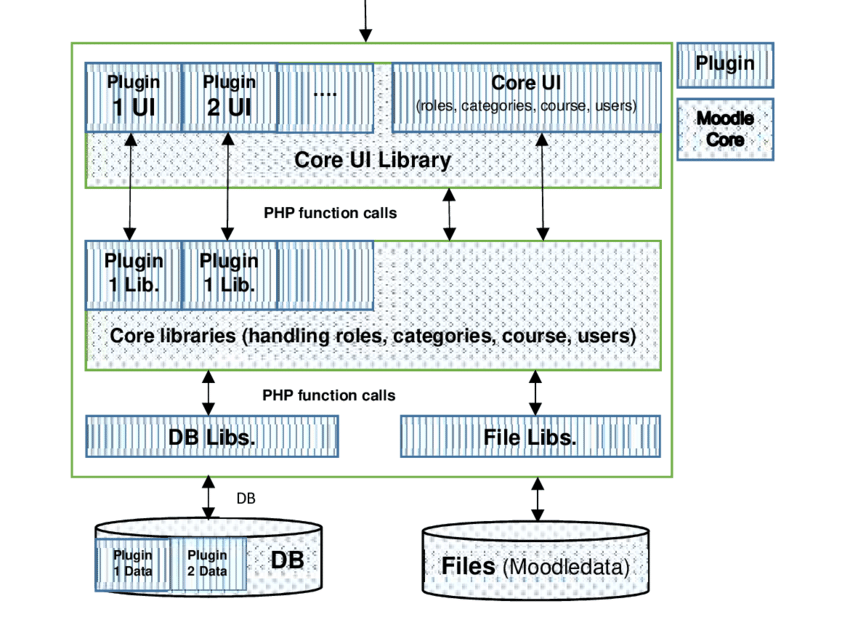
\includegraphics[width=0.8\textwidth]{images/Moodle-three-tier-architecture.png}
      \caption{Moodle three tier architecture. Source: Dolawattha et al.~\cite{dolawattha_impact_2019}.}
      \label{fig:moodle_arch}
\end{figure}

Moodle offers many plugins that allow for functionality expansion. There are
multiple types of plugins from local plugins, block plugins all the way to
antivirus plugins. Each with its own purpose and place in the moodle folder
structure.

\section{Gamification and Motivation in Education}
\noindent~Gamification is the process of applying game elements, design and mechanics to non-game contexts~\cite{deterding_gamification_2011} and when applied to higher education it demonstrated a noticeable positive effect on learning outcomes~\cite{sailer2020gamification}. However, when poorly designed and implemented, particularly when relying solely on points, badges and leaderboards without supporting intrinsic motivation, gamification can undermine student motivation~\cite{hanus2015assessing} and create anxiety through excessive competition~\cite{smiderle2020impact}.
The field faces significant methodological challenges with 50\% of studies
showing inconclusive results~\cite{dichev2017gamifying}.

\subsection{Theoretical Foundations of Gamification}
\noindent~The Self-Determination Theory (SDT) provides the dominant theoretical lens for understanding gamification effectiveness in educational contexts~\cite{deci1985intrinsic}. According to Deci and Ryan, SDT poses that human motivation stems from satisfaction of three innate psychological needs: autonomy (self-determination and willing action), competence (mastery and effectiveness) and relatedness (social connection and belongingness), The theory distinguishes between intrinsic motivation (engaging in activities for inherent satisfaction) and extrinsic motivation (from purely reward-driven to fully internalized values)~\cite{smiderle2020impact}. Ryan and Deci's later update demonstrates that autonomy-supportive environments enhance student motivation, engagement, performance and well-being across diverse cultural contexts.

The application of SDT to game design emerged with Ryan, Rigby and
Przybylski's~\cite{ryan2006motivational} work demonstrating that video game
enjoyment stems not from surface features but from need satisfaction. Ryan and
Rigby~\cite{ryan2019motivational} explicitly applied these principles to
educational contexts, arguing that game-based learning satisfies needs through
meaningful choices (autonomy), optimal challenges with clear feedback
(competence) and collaborative interaction (relatedness), while warning that
superficial gamification relying solely on extrinsic rewards threatens these
very needs.

Empirical research confirms SDT's power for gamification outcomes. Sailer et
al. experimentally tested how specific game design elements influence need
satisfaction, finding that different mechanisms satisfy different needs:
avatars and storylines increased perceived autonomy; leaderboards and
performance graphs increased perceived competence; teammates and meaningful
narratives increased perceived relatedness. Xi and Hamari~\cite{xi2019does}
demonstrated that need satisfaction mediates the relationship between
gamification features and positive outcomes, providing empirical support for
matching game mechanics to psychological needs.

Csikszentmihalyi's~\cite{csikszentmihalyi1990flow} Flow Theory complements SDT
by describing the construction of the optimal experience, complete absorptionin
an activity characterized by nine dimensions including challenge-skill balance,
clear goals, unambiguous feedback, total concentration, sense of control and
transformation of time. Flow occurs when challenges and skills are both high
and balanced, creating intrinsically rewarding experiences distinct from simple
instantaneous pleasure. The original description positioned flow as the
antidote to both boredom (when skills exceed challenges) and anxiety (when
challenges exceed skills).

The integration of SDT and Flow Theory provides a comprehensive motivational
framework: SDT explains why gamification works through need satisfaction, while
Flow Theory describes the optimal state when competence needs are met through
balanced challenge-skill dynamics, supported by autonomy and relatedness.
Proulx et al. proposed integrating learning mechanics with game mechanics under
this dual theoretical lens, distinguishing between game mechanics (rules and
procedures) and learning mechanics (pedagogical strategies) while ensuring
alignment with psychological need satisfaction.

\subsection{Gamification Mechanics}
\noindent~The critical factor determining whether gamificatin supports or undermines motivation appears to be implementation approach. Koivisto and Hamari~\cite{koivisto2019rise} reviewed gamification research and indentified a gap between promise and practice, noting that the most effective implementations are grounded in motivational theory rather than superficial application of game elements.

Leaderboards exemplify gamification's most controversial element driving
engagement for some learners while creating anxiety and demotivation for
others. Li and Fryer's~\cite{li2024leaderboards} systematic review of empirical
evidence in higher education concluded that leaderboards remain amongst the
most popular gamification elements but should be used with clear ranking rules
and goal-related feedback to avoid detrimental effects. Leaderboards may
benefit high-performing students but have negative consequences for
underperforming ones, shifting focus from learning to ranking.

Points systems represent the most fundamental gamification mechanic, providing
immediate quatitative feedback for actions and achievements. Park and
Kim~\cite{park2022points} distinguished between qualitative points (high/low
scores displayed on leaderboards) and quantitative points (accumulative
token-like currencies), noting that points are the most widely used game
mechanics but improper use causes learners to focus on earning points without
genuine learning purpose.

Despite criticisms, well-designed points systems demonstrate usefulness.
Experience points (XP) and leveling systems create a sense of continuous
progress by providing granular feedback that makes small actions worthwhile.
Paiva et al.~\cite{paiva2015badges} found that XP systems combined with badges
created a sense of constant progress, proving powerful in learning applications
where skill development occurs incrementally.

Progress bars and visual feedback leverage what Park and
Kim~\cite{park2022points} identify as the Zeigarnik effect, the psychological
need to complete unfinished tasks. They provide immediate visual feedback that
makes abstract advancement concrete and visible.

When properly implemented, with theorectical rigor, gamification demonstrates
genuine potential to enhance cognitive, motivational and behavioral outcomes.
The challenge for higher education is moving beyond the superficial
implementation toward sophisticated applications that follow what motivational
psychology teaches about human learning and development.

\chapter{The Learning Scorecard: Concept and Evolution}
\section{Genesis and Conceptualization of the Learning Scorecard}
\noindent The Learning Scorecard emerged from a fundamental pedagogical challenge identified within higher educational institutions: the lack of understanding by faculty members regarding the difficulties experienced by students in relation to the content taught in curricular units as well as the students lack motivation in respect to the academic autonomous work. Initially, this platform was conceptualized as an academic performance management system designed to support both students and faculty through data-driven insights that assist teachers in continuously monitoring the curricular units they teach while enabling students to visualize their performance in each course in which they are enrolled. Their main mission was to offer higher education students an analytic environment that allows progress monitorization through a familiar game-like scope, contributing for a better learning experience.

The platform was originally conceptualized with three distinct user
perspectives: student view, teacher view and administrative view. The student
view provides essential visualizations that enable students to understand their
learning trajectory in a specific curricular unit while offering tools that
provide important data for continuous monitoring by faculty. The teacher view
provides management, evaluations and visualization tools for educators
regarding each curricular unit they teach, offering various visualizations to
track the collective students progress through all phases of the curricular
unit along with assessment tools.

\section{Evolution Through Iterative Development}
\subsection{Historical Overview of Versions}
\noindent The Learning Scorecard concept began in the 2015/16 academic year as a collaborative project project undertaken by a group of Computer Science masters students enrolled in the Information Systems of Decision Support II curricular unit under the advice of Prof.~Elsa Cardoso. This group defined in a very basic and introductory way what the LS would be, later being picked up by Daniela Costa~\cite{costa_thesis_2017} who built upon this concept, improving it and setting the course for the following iterations..

The development timeline reflects the progression of features and refinements
with each major version addressing specific limitations and opportunities
identified through previous implementations. This iterative approach has
enabled the platform to evolve in response to changing technological
landscapes, pedagogical insights and institutional requirements while
maintaining consistency in core design principles.

\textbf{Learning Scorecard Version 0}

\noindent The inaugural version of the Learning Scorecard was developed by Daniela Costa as part of her master's dissertation at ISCTE-IUL~\cite{costa_thesis_2017}, whose primary objective was to create a web-based platform that would integrate Business Intelligence techniques with gamification elements in order to foster improved student learning experiences in higher education contexts.

This version adopted conventional three-tier web application architecture,
comprising distinct presentation, application and data layers. This
architectural pattern, while traditional, provided a stable foundation for the
initial implementation and facilitated separation of concerns accross system
components.

The presentation layer was constructed using fundamental web technologies
including HTML5, CSS3 and JavaScript. The Bootstrap
framework\cite{bootstrap_framework} was incorporated to ensure responsive
design principles and provide pre-built user interface components.
Chart.js~\cite{chartjs_org}, a JavaScript visualization library, was integrated
to facilitate the creation of interactive dashboard and data visualizations,
essential for performance monitoring. The application layer was built upon
Node.js, with Express.js as the web application framework, providing routing
capabilities and middleware integration. MySQL~\cite{mysql_database} was
selected as the relational database management system (RDBMS), choosen for its
compatibility with Node.js's~\cite{nodejs_org} asynchronous architecture and
its widespread adoption in academic environments. The database schema was
designed to accommodate user profiles, course information, assessment data and
gamification elements.

This platform was deployed in the SIAD I (Data Warehouse and Business
Intelligence) course during the 2016/2017 academic year. Comparative analysis
with the previous academic year (2015/2016, without LS implementation) revealed
statistically significant improvements accross multiple performance indicators.
The approval rate of students increased from 86\% to 92\%, the mean grade
improved from 13.25 to 13.74 (on a 0-20 scale), the number of failed students
decreased from 17 to 10 students and the number of students that withdrew from
the course also decreased from 21 to 12 students.

Post-implementation analysis revealed several technical and functional
limitations, such as the absence of proactive notification mechanisms for
approaching quest deadlines, limited diversity in quiz question formats and
assessment types, code modularity deficiencies impeding extensibility,
scalability constraints when supporting large concurrent user populations and
suboptimal code organization affecting maintainability.

\textbf{Learning Scorecard Version 1}

\noindent Version 1 represented an evolutionary refinement of the Learning Scorecard developed collaboratively by Francisco Rações and Tiago Pedroso during the 2017/2018 academic year. Rather than representing a single unified dissertation, their work constituted two complementary master's research projects that addressed distinct but interconnected dimensions of the Learning Scorecard: systematic gamification enhancement through theoretical frameworks (Pedroso) and advanced information visualization and dashboard design (Rações).

The primary motivation driving version 1 development stemmed from identified
limitations in version 0 and broader challenges in educational gamification and
learning analytics.

Educational gamification implementations frequently suffer from superficial
application of game elements, often limited to points, badges and leaderboards
(PBL), without systematic consideration of how these mechanics connect to
student motivation and desired learning outcome. Pedroso's focus was to analyze
how gamification can be systematically designed to enhance student's engagement
and motivation. Rações however, focused on how student learning progress in
higher education courses is typically not monitored in real-time. His
contribution was mainly on students perception of their learning progress
through well-designed dashboards and visualization techniques.

This version maintained and incrementally enhanced the core technological
foundation estabilished in version 0 with the key technical enhancements being:
(1) expanded data collection mechanisms for additional learning indicators; (2)
enhanced dashboard rendering capabilities, supporting more complex
visualizations; (3) improved gamification element tracking and state
persistence; (4) refined user interface components with a more responsive
design and (5) optimized database queries for performance improvements.

The central theoretical innovation of version 1 was Pedroso's systematic
application of the MDA (Mechanics, Dynamics, Aesthetics) framework proposed by
Hunicke, Leblanc and Zubek~\cite{hunicke_mda_2004}. The MDA framework
represents a formal approach to game design and game research, providing an
analysis methodology for understanding how game elements interact and how they
can be applied outside traditional gaming contexts.

\begin{figure}[H]
      \centering
      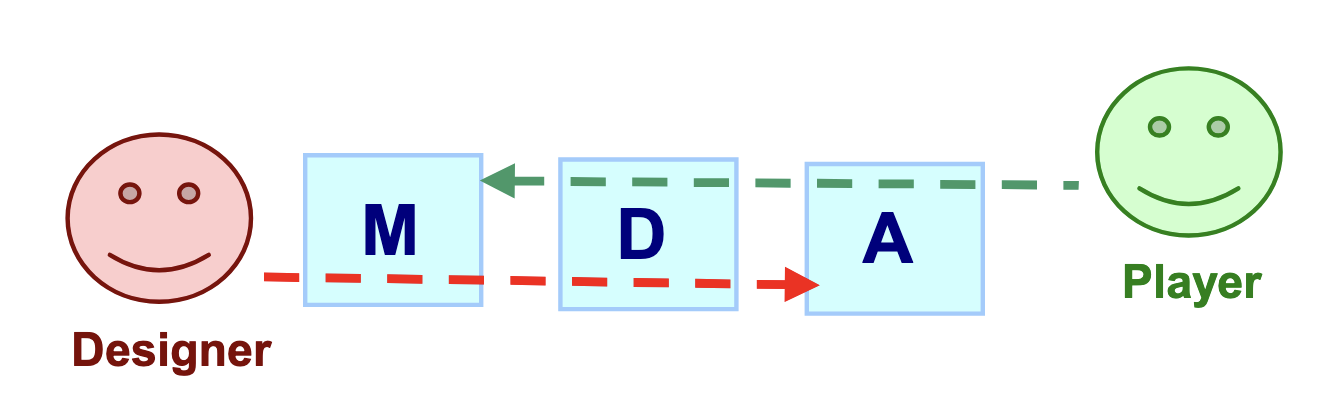
\includegraphics[width=0.8\textwidth]{images/mda-perspectives.png}
      \caption{MDA Perspectives. Source: Hunicke R. et al.~\cite{hunicke_mda_2004}.}
      \label{fig:mda-perspectives}
\end{figure}

Following the MDA framework, Pedroso designed and implemented gamification
mechanics intended to generate specific dynamics and aesthetic outcomes.
\begin{comment}
\\TODO SPACING
\end{comment}

\textbf{Implemented Mechanics}
\begin{enumerate}
      \item[1.] Experience Points (XP) System
            \begin{itemize}
                  \item Awarded for completion of learning activities (quizzes, assignments, etc.).
                  \item Cumullative XP tracking throughout the semester.
                  \item Transparent XP calculation rules communicated to students.
            \end{itemize}
      \item[2.] Badge System
            \begin{itemize}
                  \item Achievement recognition for specific accomplishments.
                  \item Categories: content mastery, participation, consistency and excellence.
                  \item Visual representation with iconography.
                  \item Badge collection displayed in student profiles.
            \end{itemize}
      \item[3.] Leaderboard
            \begin{itemize}
                  \item Ranked display of student performance based on XP.
                  \item Multiple leaderboard views (class-wide, groups, etc.).
                  \item Regular updates maintaining current standings.
            \end{itemize}
      \item[4.] Quest System
            \begin{itemize}
                  \item Structured learning activities with clear objectives and deadlines.
                  \item Multiple quest types: practical assignments, exercises, quizzes and forum
                        discussions.
                  \item Progress tracking with completion status visualization.
                  \item XP rewards tied to quest completion and quality.
            \end{itemize}
      \item[5.] Level System
            \begin{itemize}
                  \item Hierarchical progression indicators based on cumulative XP.
                  \item Level thresholds established to create meaningful advancement milestones.
                  \item Level-up notifications providing motivational reinforcement.
                  \item Visual representation of current level and progress toward next level.
            \end{itemize}
      \item[6.] Progress Visualization
            \begin{itemize}
                  \item Dashboards showing advancement through course content.
                  \item Timeline representations of quest deadlines and completion.
                  \item Comparative visualizations (individual vs. class average).
            \end{itemize}
\end{enumerate}

\textbf{Targeted Dynamics}
\begin{itemize}
      \item Competition: Leaderboards and public XP totals create competitive motivation
            between students.
      \item Progression: Level advancement provides clear sense of forward movement.
      \item Goal-Orientation: Quest structures with defined objectives focus student
            effort.
      \item Social Comparison: Peer performance visibility enables self-assessment in
            context.
      \item Achievement Recognition: Badges provide symbolic acknowledgement of
            accomplishments.
      \item Time Management: Quest deadlines encourage consistent engagement rather than
            cramming.
\end{itemize}

\textbf{Intended Aesthetics}
\begin{itemize}
      \item Challenge: Encouraging mastery through structured, progressively difficult
            learning objectives.
      \item Discovery: Facilitating exploration of course content and connections between
            concepts.
      \item Progression: Providing clear sense of advancement and competence development.
      \item Fellowship: Creating awareness of collective class journey and peer community.
      \item Narrative: Structuring semester as coherent learning journey milestones.
\end{itemize}

Rações's contributed mainly by developing comprehensive dashboard interfaces
for both students and faculty and by indentifying and implementing core
learning indicators categorized in three dimensions: engagement indicators,
coginitive indicators and social indicators.

Engagement indicators measured the interactions with the learning contents,
frequency of access to the platform and submission timeliness. Whereas
cognitive indicators tracked grade and performance trends, quiz attempts before
achieving success, performance consistency and improvement trajectories. The
social indicators provided a measure on forum posting frequency and
consistency, peer interaction patterns and collaborative activity participation
and contribution quality.

In regards to the dashboards, he made improvements on the students view
providing actionable insights while focusing on information clarity through
visualization components such as:
\begin{itemize}
      \item Line charts tracking temporal patterns of engagement (platform access and forum
            activity over weeks).
      \item Bar charts for comparing quiz grades across multiple assessments.
      \item Radar charts for multi dimensional performance profiling.
      \item Progress indicators as a visual representation of quest completion and level
            advancement.
      \item Tables with detailed statistical breakdowns of quiz performance and attempt
            histories.
\end{itemize}

\begin{figure}[H]
      \centering
      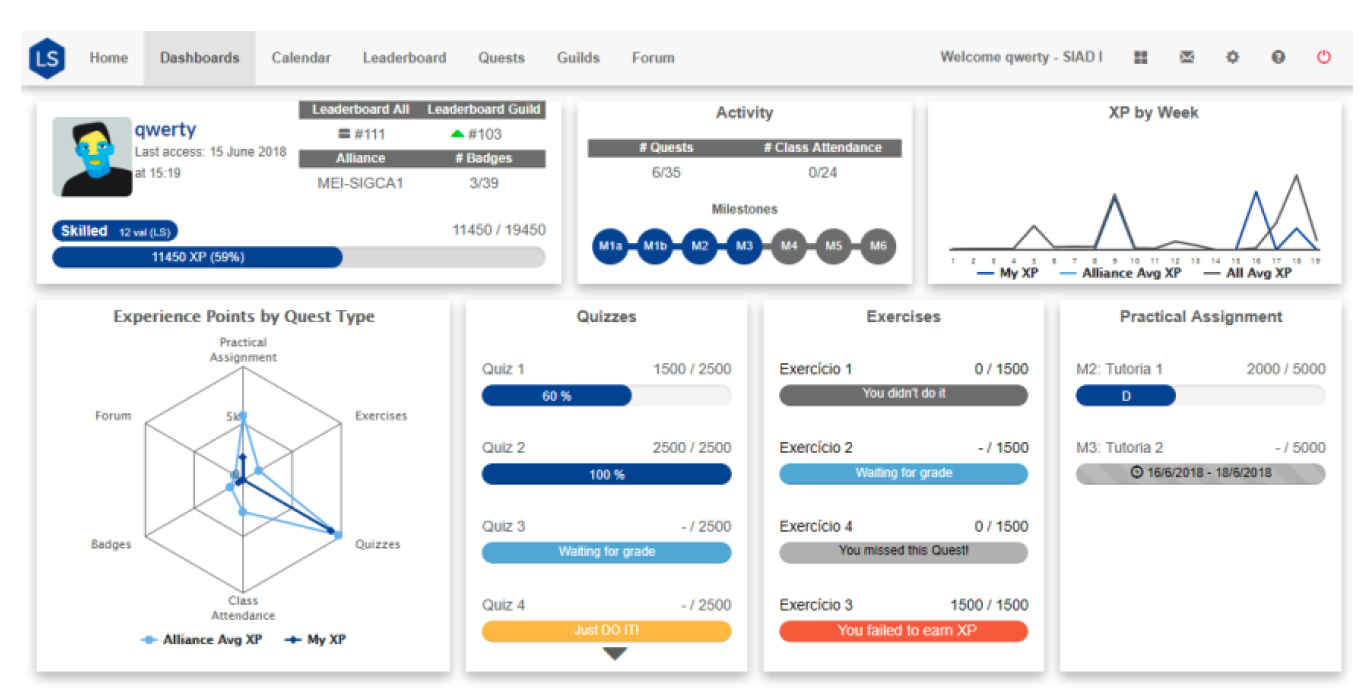
\includegraphics[width=0.8\textwidth]{images/student-dashboard-v1.png}
      \caption{Student Dashboard (Version 1). Source: Rações F.~\cite{racoes_thesis_2018}.}
      \label{fig:student-dashboard}
\end{figure}

On the faculty view, he designed the dashboards according to Business
Intelligence best practices for analytical decision support with the following
key metrics being displayed:
\begin{itemize}
      \item Number of active vs.\ inactive students.
      \item Average quiz grades with trend indicators.
      \item Forum participation rates across the entire class.
      \item Assignment submission delay distributions.
      \item At-risk student identification based on multiple indicator thresholds.
\end{itemize}

\begin{figure}[H]
      \centering
      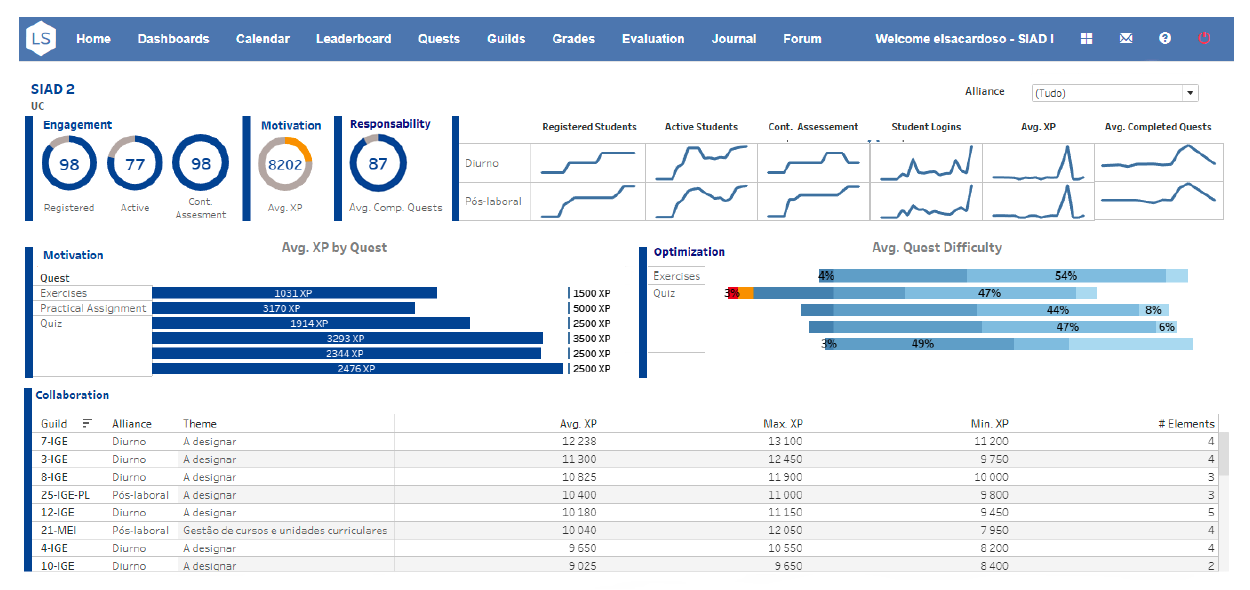
\includegraphics[width=0.8\textwidth]{images/teacher-dashboard-v1.png}
      \caption{Teacher Dashboard (Version 1). Source: Rações F.~\cite{racoes_thesis_2018}.}
      \label{fig:teacher-dashboard}
\end{figure}

Version 1 was deployed during the 2017/2018 academic year at ISCTE-IUL in two
courses: SIAD I (first semester) and SIAD II (second semester). This
represented the platforms third and fourth consecutive semester deployments,
building upon the foundation established the previous academic year.

Despite significant advances, this version retained limitations, motivating
future development and iteration:
\begin{itemize}
      \item Technical Limitations
            \begin{itemize}
                  \item Code Modularity: While improved over version 1, codebase still exhibited
                        architectural constraints limiting extensibility
                  \item Scalability Concerns: Performance characteristics with large user populations
                        remained uncertain
                  \item Data processing: Some analytics required manual calculation or batch processing
                        rather than real-time computation
            \end{itemize}
      \item Functional Limitations
            \begin{itemize}
                  \item Difficuty Assessment: Lacking mechanisms to capture student-perceived
                        difficulty of content topics
                  \item Adaptive Learning: Limited capability to personalize learning paths based on
                        individual student characteristics
                  \item Predictive Analytics: No predictive modeling of future student and class
                        performance
            \end{itemize}
      \item Pedagogical Considerations
            \begin{itemize}
                  \item Self-Reported Data: Reliance on faculty to input the information regarding
                        students grades, performance, etc.
                  \item Generalizability: Implementation validated in SIAD courses, applicability to
                        other courses uncertain
            \end{itemize}
\end{itemize}

While version 1 achieved significant pedagogical and user experience
improvements, these identified technical and functional limitations motivated
Miguel Lopes'~\cite{lopes_ontologies_2021} subsequent comprehensive
architectural reimagination (version 2), which would address scalability
concerns and integrate semantic web technologies while preserving the
gamification and visualization innovations contributed by Pedroso and Rações.

\textbf{Learning Scorecard Version 2}

The latest version of Learning Scorecard, version 2, developed by Miguel
Lopes~\cite{lopes_ontologies_2021} during the 2020/2021 academic year at
ISCTE-IUL. This version constituted a complete platform redevelopment rather
than incremental enhancement, motivated by critical limitations that had
accumulated across three previous iterations.

Lopes'~\cite{lopes_ontologies_2021} key contributions to this version were the
implementation of a semantic web through the application of ontologies and
integration of a GraphQL~\cite{graphdb_ontotext} semantic database, the
application of a structured mechanism for continuous student feedback on
learning difficulties and a shift from the monolithical three tier architecture
into a cloud-native, microservices design that enabled scalability and
multi-institutional deployment.

In this version, the sylabus contents could be stored in the GraphDB database
and displayed to the students as a better way to visualize the course's
contents as shown in figure~\ref{fig:sylabus-uc}.

\begin{figure}[H]
      \centering
      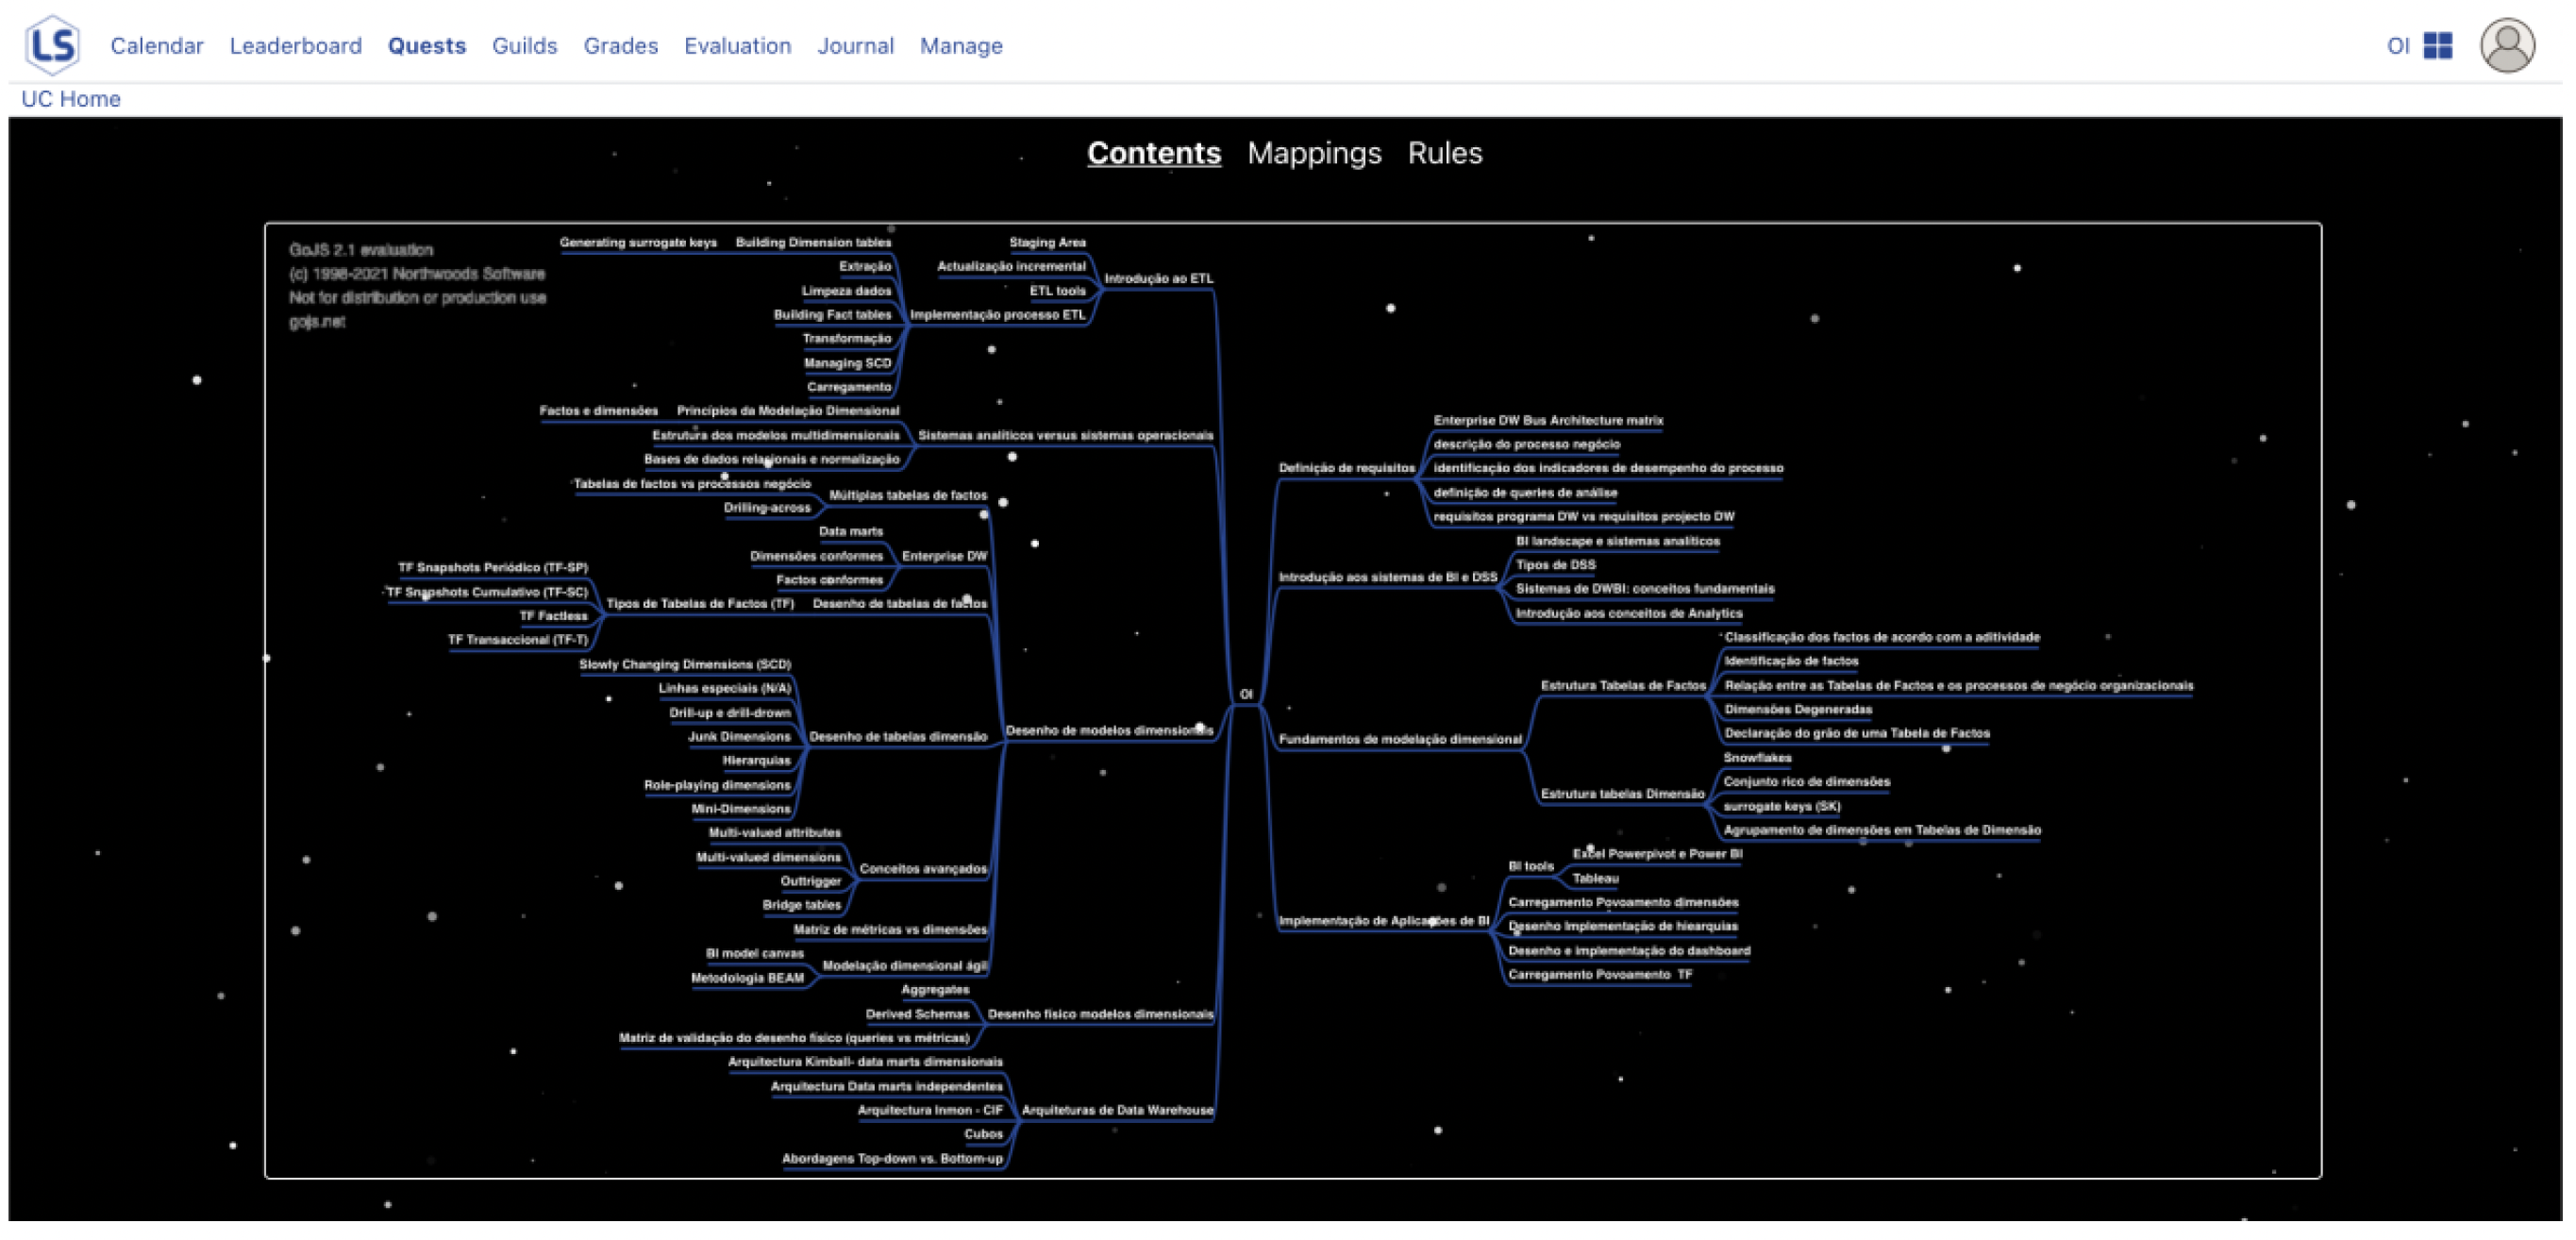
\includegraphics[width=0.8\textwidth]{images/sylabus-uc-v2.png}
      \caption{Sylabus Contents of an UC. Source: Lopes M.~\cite{lopes_ontologies_2021}.}
      \label{fig:sylabus-uc}
\end{figure}

The learning difficulties of students could be gathered through a questionnaire
after every quest (see figure~\ref{fig:quest-validation}), presented to
students as a quest validation that would give the quests XP upon completion.
This would provide the faculty a better view of the students challenges and
feedback on the lessons, as well as what needed to be revised as demonstrated
in the figure~\ref{fig:sylabus-uc-with-validation}.
\begin{figure}[H]
      \centering
      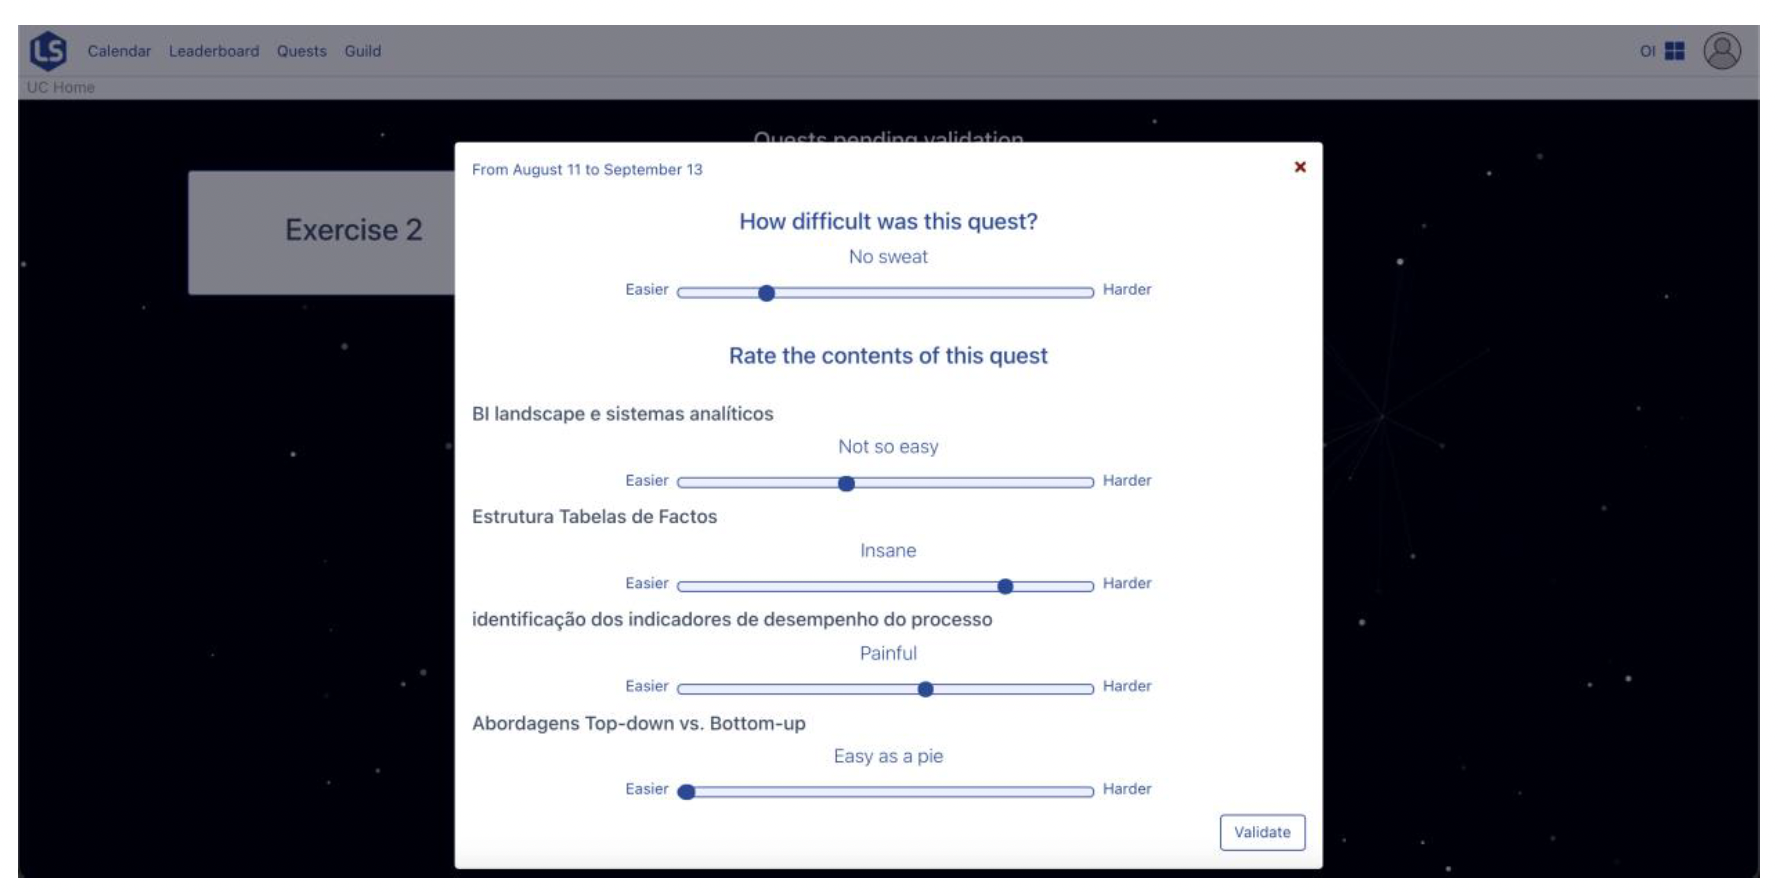
\includegraphics[width=0.8\textwidth]{images/difficulty-tab-v2.png}
      \caption{Difficulty questionnaire (quest validation). Source: Lopes M.~\cite{lopes_ontologies_2021}.}
      \label{fig:quest-validation}
\end{figure}

\begin{figure}[H]
      \centering
      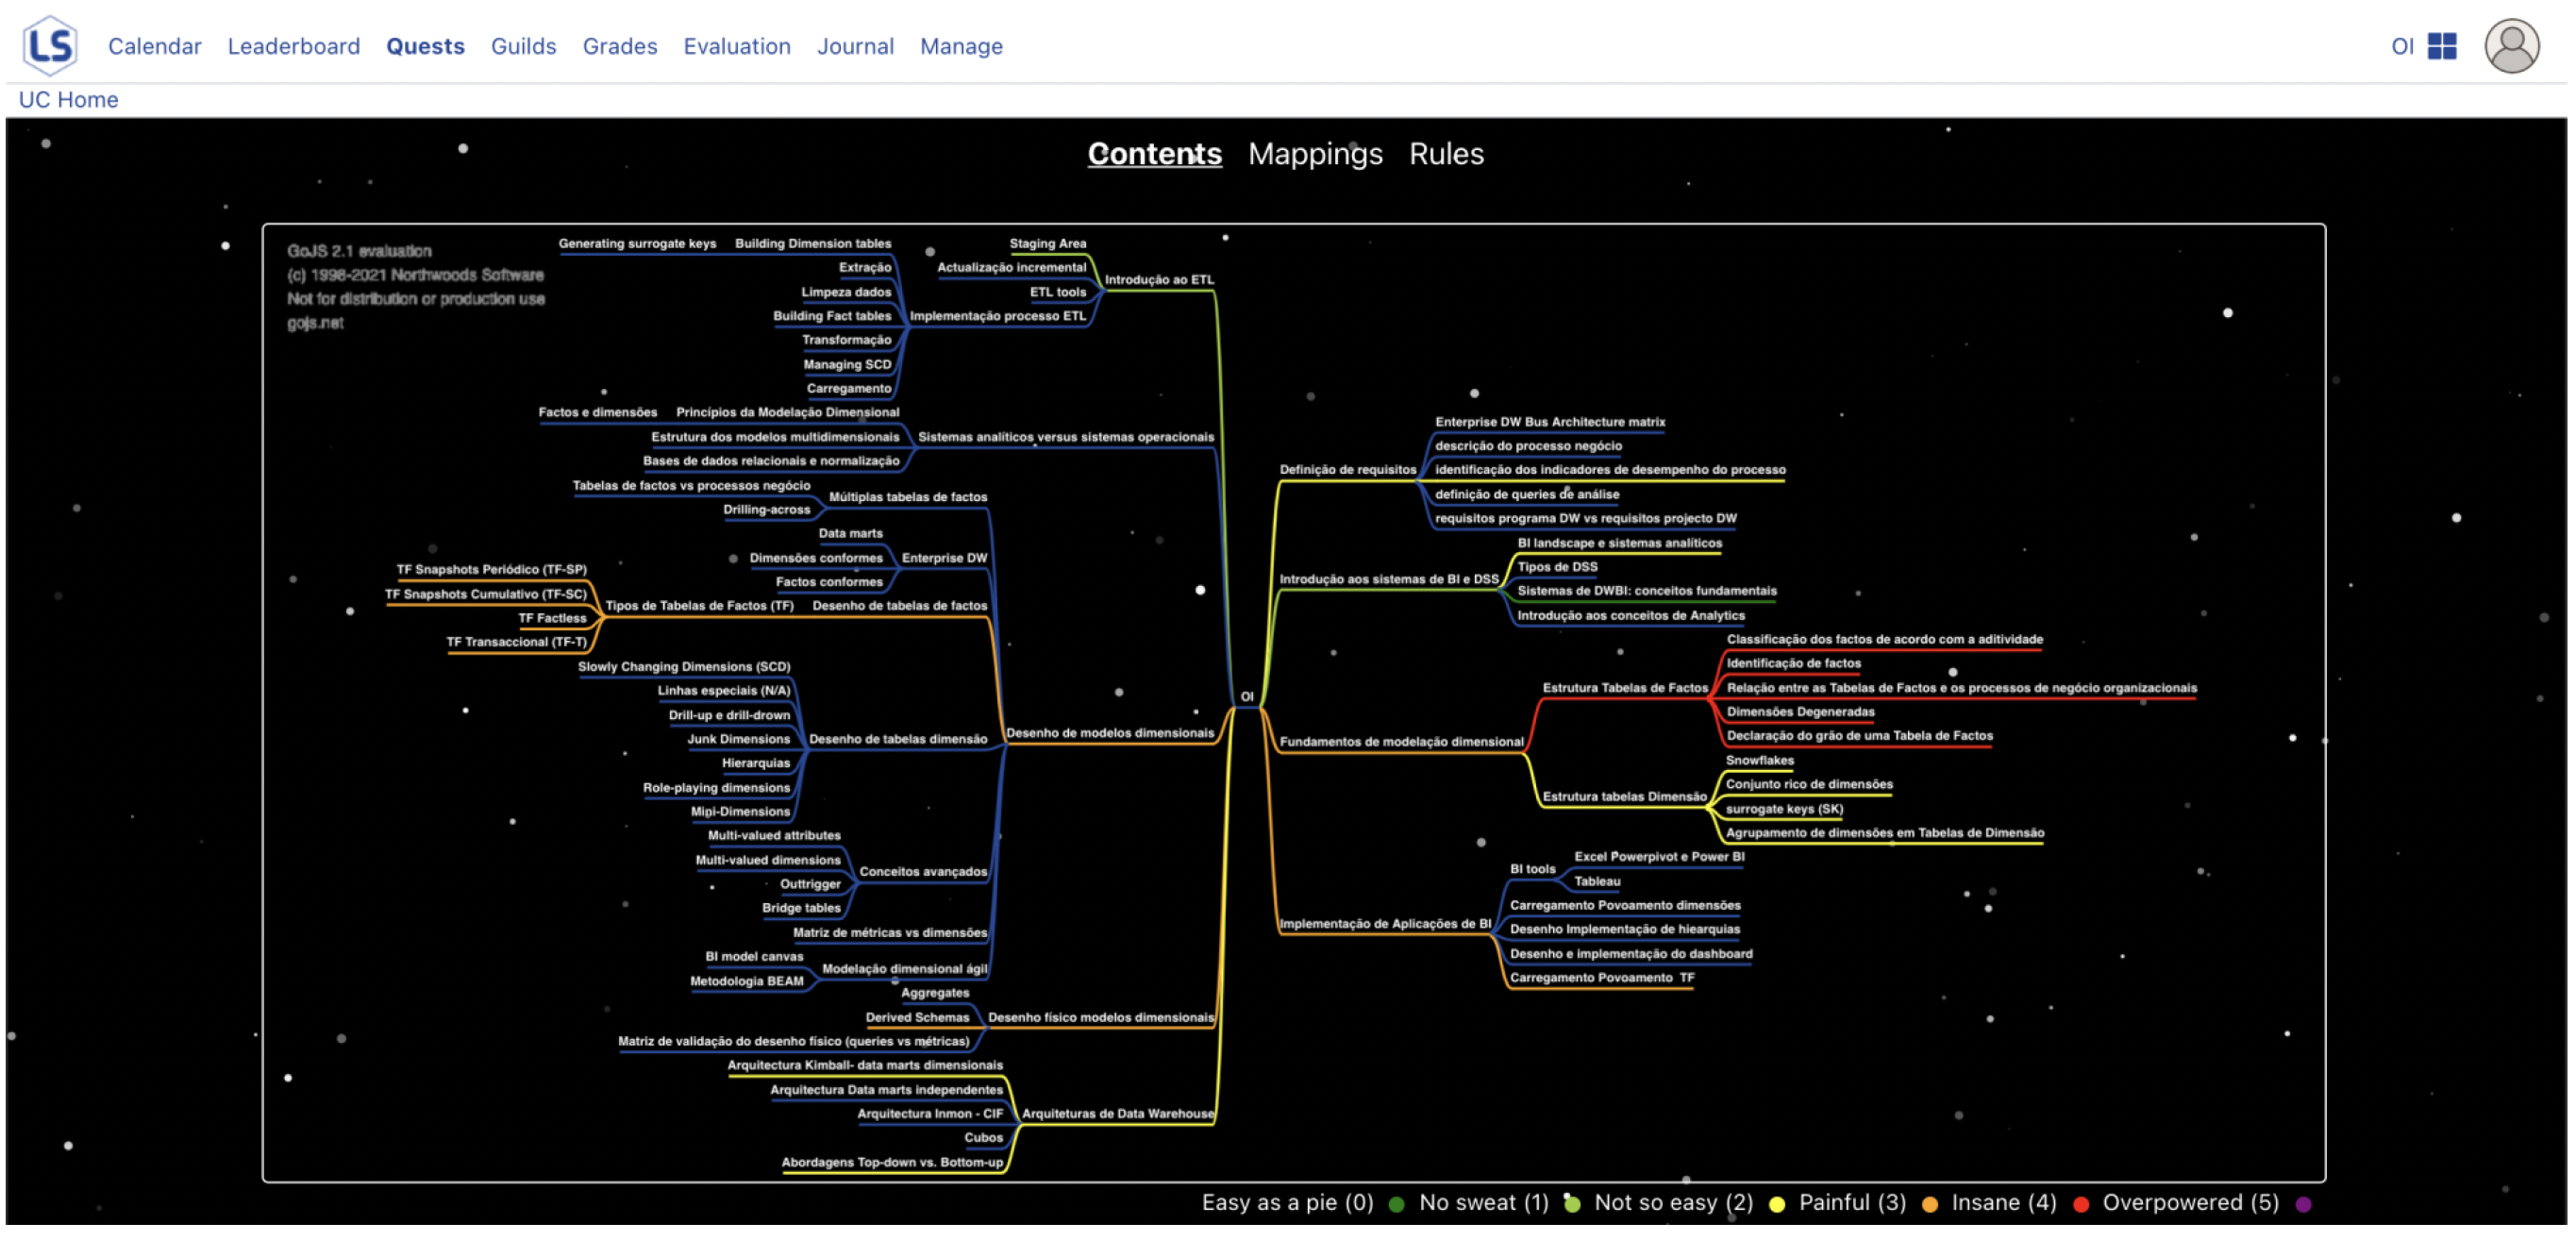
\includegraphics[width=0.8\textwidth]{images/sylabus-uc-with-difficulty-v2.png}
      \caption{Syllabus contents with difficulty perceived by students. Source: Lopes M.~\cite{lopes_ontologies_2021}.}
      \label{fig:sylabus-uc-with-validation}
\end{figure}

Further technical investigation will come when analyzing the current state of
the application in chapter 4 of this dissertation.

\subsection{Lessons Learned from Prior Iterations}

The evolutionary development of the Learning Scorecard has yielded important
insights into the challenges and opportunities associated with educational
technology implementation in higher education contexts. These lessons have
directly informed the design decisions underlying Learning Scorecard 3.0 and
provide valuable guidance for future LS development efforts.

Previous iterations consistently revealed the critical importance of seamless
integration with existing institutional systems and workflows. Standalone
implementations, while providing flexibility and autonomy, created barries to
adoption through the requirement for separate authentication, manual data entry
and navigation between multiple platforms. These experiences highlighted the
need for deeper integration with institutional learning management systems to
achieve sustainable adoption and effectiveness.

Analysis of user behavior accross previous versions revealed important patterns
regarding the factors that drive sustained engagement with educational
technology platforms. Students demonstrated higher levels of engagement when
gamification elements were seamlessly integrated with existing academic
workflows rather than requiring separate platform visits or additional effort
investment. Faculty adoption correlated strongly with the availability of
actionable insights that directly supported pedagogical decision-making without
creating additional workload or administrative burden.

The operational experience of maintaining standalone Learning Scorecard
implementations revealed significant challenges related to infrastructure
costs, security management and version compatibility. These experiences
demonstrated the advantages of leveraging existing institutional infrastructure
and support systems rather than maintaining separate technological stacks that
require independent updates, security monitoring and user support.
\section{Learning Scorecard Conceptual Framework}

The Learning Scorecard (LS) conceptual framework encompasses a comprehensive
set of interconnected concepts designed to support gamified learning
experiences in higher education. This framework is organized around four
primary domains that reflect different aspects of the educational experience:
Academic Structure and Organization, Gamification Mechanics, Social Learning.
These concepts can be organized into four primary domains: Academic Structure,
Gamification Mechanics, Social Learning and Recognition and Achievement
Systems. Each domain contains interconnected concepts that work together to
create a comprehensive educational technology ecosystem that supports both
individual learning, cooperation and institutional objectives.

\subsection{Academic Structure and Organization}

The academic foundation of the Learning Scorecard is built upon traditional
higher education organizational structures, adapted to support digital learning
environments.

\textbf{Courses and Curricular Units.} The system recognizes a two-tier academic structure where \textit{Courses} represent overarching academic programs (e.g., "Computer Science") that encompass multiple \textit{Curricular Units}. Each Curricular Unit corresponds to an individual subject with specific learning objectives, content and assessments that students must complete as part of their academic progression. This hierarchical organization maintains consistency with traditional academic frameworks while enabling digital tracking and gamification.

\textbf{Students and Faculty.} The system accommodates two primary user roles: \textit{Students}, who are enrolled in one or more Curricular Units and participate in gamified learning activities and \textit{Teachers} or Faculty members, who are responsible for creating and managing curricular content, designing learning activities and monitoring student progress within their assigned Curricular Units.

\textbf{Syllabus Contents, Calendar and Timeline.} \textit{Syllabus Contents} encompass all learning materials, resources and educational content within a Curricular Unit. The organizational framework includes both \textit{Calendar} and \textit{Timeline} concepts that serve as complementary planning systems, enabling students and faculty to organize learning activities and maintain temporal awareness of curricular progression.

\subsection{Gamification Mechanics}

The core gamification elements provide the foundation for student engagement
and progress tracking through game-like mechanics adapted to educational
contexts.

\textbf{Experience Points and Ranks.} \textit{Experience Points} (XP) serve as the fundamental currency of progress within the platform, earned through completion of various educational activities. The \textit{Rank} system establishes hierarchical progression levels based on accumulated XP, including ranks such as Newbie (entry level at 0 XP), Rookie, Skilled Expert, Master and Legendary. Faculty members can configure rank thresholds dynamically, with each rank unlocking new privileges and recognition within the platform.

\textbf{Quests.} \textit{Quests} represent the core educational activities that students complete to earn XP and demonstrate learning. The system categorizes quests into five distinct types: Class Attendance, Practical Assignment, Quiz, Exercise and Event. Each quest can be designated as mandatory (milestone quests) or optional, providing flexibility in curriculum design while maintaining educational objectives.

\textbf{Last Chances.} The \textit{Last Chance} mechanism provides opportunities for recovery and continued engagement when students fall behind or make mistakes, preventing permanent failure states that could lead to disengagement and ensuring continued participation throughout the academic term.

\subsection{Social Learning}

The social components of the Learning Scorecard foster collaboration and
healthy competition among students through structured group dynamics.

\textbf{Alliances.} \textit{Alliances} function as large-scale organizational units that typically correspond to academic classes or programs (e.g., LEI or ETI). These structures facilitate competition and comparison at the class level while maintaining educational coherence, enabling students to compare their progress through dedicated leaderboards and participate in alliance-specific activities.

\textbf{Guilds.} \textit{Guilds} represent smaller collaborative units within alliances, typically corresponding to project teams or study groups. The guild system promotes cooperative learning by encouraging mutual assistance among members, with guild-specific achievements, badges and leaderboards fostering team spirit while maintaining individual accountability within the collaborative framework.

\subsection{Recognition and Achievement System}

The recognition framework provides multiple pathways for acknowledging student
accomplishments and maintaining motivation through visible achievements.

\textbf{Badges.} The \textit{Badge} system provides targeted recognition for specific accomplishments and behaviors, featuring 39 different badges organized into four categories: individual achievements, guild-based accomplishments, forum participation and final questionnaire completion. Each category includes multiple tiers (bronze, silver, gold and platinum) corresponding to increasing levels of difficulty and commitment.

\textbf{Trophies.} \textit{Trophies} represent the highest level of achievement, awarded to top performers in various leaderboard categories including overall rankings (Best Score Player), guild performance (Best Guild) and combined metrics (Best Triathlon Player). Each trophy provides substantial XP rewards (typically 1000 XP) and serves as a highly visible symbol of excellence.

\textbf{Avatars.} The \textit{Avatar} system enables profile customization while serving as a visual indicator of progression. Students unlock new avatar options as they advance through rank levels, with both male and female options available at each tier, allowing for personal expression while maintaining the connection between visual representation and academic achievement.

\textbf{Leaderboards.} Multiple \textit{Leaderboard} systems enable various forms of competition and comparison through five distinct categories: overall individual rankings, guild-based comparisons, exercise-specific performance, quiz results and combined metrics. Each leaderboard displays position, username, rank, avatar and XP totals, creating transparency in academic performance while fostering healthy competition among participants.

\chapter{System Architecture and Design}
\section{Requirements}
\noindent An imperative aspect in any application conceptualization is a thorough requirement analysis. These requirements can be functional (FR) or non functional (NFR) and shape the architectural decisions that are made during its development as well as assessing whether a system will succeed.

\textbf{Functional Requirements (FR)}

It's important to define what an engineer should strive for when determining
functional requirements as it will ultimately be what defines an application,
molds its functionality and consequently decides it's architecture. Functional
requirements are the essential characteristics that the system should deliver
that the end-user specifically demands.~\cite{saroja_functional_2023} A simpler
way to perceive it is that they define what the system should perform. It's
important with any version increment of the LS to maintain fidelity to the
previous requirements and adjust them when appropriate.
Costa~\cite{costa_thesis_2017} identified base functional requirements which I
will evaluate and integrate into my system architecture, but also define some
myself.
\begin{enumerate}
      \item[FR1] The LS platform must use Moodle's existing authentication and user
            management systems.
      \item[FR2] The LS platform must be integrated with the e-learning system, providing
            seamless access to student data, course data and activities.
      \item[FR3] The LS Platform must use Moodle's role-based access control mechanisms,
            distinguishing between student and teacher user types with corresponding
            permissions and interfaces.
      \item[FR4] The LS platform must have a dashboard for individual student performance
            monitorization (students view)
      \item[FR5] The LS platform must have a dashboard for class performance monitorization
            (teacher view)
      \item[FR6] The LS platform must have a course chronogram with deadlines and study
            guidelines, personalized by the teacher/faculty
      \item[FR7] The LS platform must include gamification elements (score, ranks, quests,
            leaderboards)
\end{enumerate}

\textbf{Non-Functional Requirements (NFR)}

Another important aspect of the requirement analysis is to define the
non-functional requirements. These, differently from their functional
counterpart must define how the system should perform, rather than what. While
not directly visible as features they are vital in shaping the user experience
and ensuring the system's long-term success. A few examples of these
requirements could be performance, security, reliability, etc.
Costa~\cite{costa_thesis_2017} also layed out base non-functional requirements
which I will also evaluate, adapt and integrate into my system architecture, in
addition to some identified by myself. From Costa's non-functional
requirements:
\begin{enumerate}
      \item[NFR1] Portability for the different web browsers, including mobile devices
      \item[NFR2] Intuitive and user-friendly interface (least possible manual input by
            students)
      \item[NFR3] The user identification data must be private (ethical requirement), the
            teacher/faculty must only have access to the class agregated data, even for at
            risk students.
\end{enumerate}
This last non-functional requirement, as Costa~\cite{costa_thesis_2017} correctly identified is a missed opportunity as the faculty will have no way of knowing which student is at risk and ultimately take advantage of such introspective metrics on student performance. As the system is integrated into moodles learning environment and all this information is already available to the faculty I believe this NFR should be altered into a more transparent requirement and only require anonymization of students the data if the Learning Scorecard extended its functionality to allow for a predictive model to be set in place to predict the outcome of the students grade based on current effort. Therefore, the corrected NFR3 is:
\begin{itemize}
      \item[NFR3] The user identification data must be private (ethical requirement) in
            case it's used in colaboration with a predictive model for the grades. The
            teacher must only have access to the class agregated data.
\end{itemize}

Throughout the study and conceptualization of the system a few more
non-functional requirements were identified:
\begin{enumerate}
      \item[NFR4] The system must be installable as standard Moodle plugin(s) without
            requiring server modification.
      \item[NFR5] The system must maintain visual consistency with the Moodle theme.
      \item[NFR6] The system must store all data within the Moodle database structure.
\end{enumerate}
\section{Overview of LS Architecture}
\subsection{Evolution from Standalone Architecture}
\noindent The LS architecture has withstood many iterations throughout the years and has become more complex and polished through them, as new features have been added, alternatives and changes in architecture have been thought as most adequate. Let's suppose we take the latest version as a baseline and dive into what can be improved.

In the latest version of the Learning Scorecard, version 2.0, as documented by
Miguel Lopes~\cite{lopes_ontologies_2021} the technological stack consisted of
React~\cite{react_dev} frontend components communicating with
Express~\cite{express_js} (NodeJS~\cite{nodejs_org}) backend services, which in
turn interfaced through REST with a cloud-hosted NoSQL MongoDB
database~\cite{mongodb_database} and GraphDB~\cite{graphdb_ontotext} system
deployed in Azure infrastructure~\cite{azure_microsoft} primarily hosted in
Heroku~\cite{heroku_platform}.
\begin{figure}[H]
      \centering
      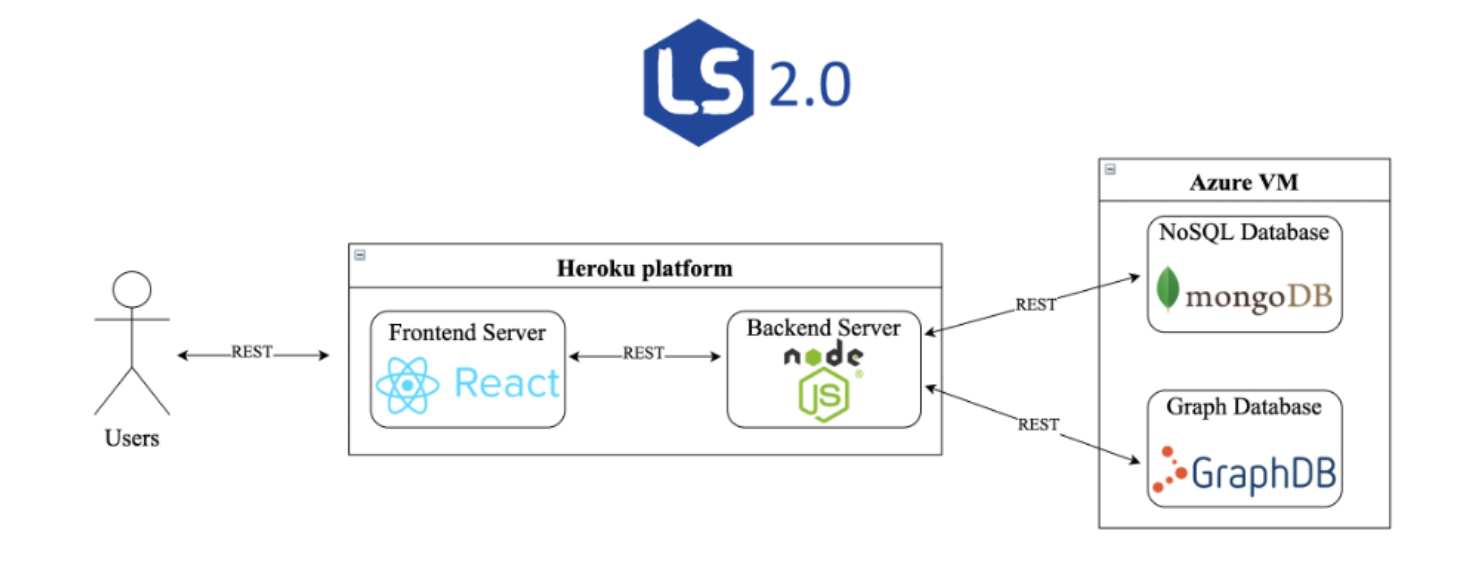
\includegraphics[width=0.8\textwidth]{images/LS2Architecture.png}
      \caption{LS 2.0 architecture. Source: Lopes M.~\cite{lopes_ontologies_2021}.}
      \label{fig:ls2_arch}
\end{figure}

While this architecture demonstrated scalabilty, modularity and adherence to
modern web development practices, it presented several critical limitations,
mainly in the fact that it is not integrated with the ISCTE Moodle environment
(FR2), relying on manual input by the faculty and students making it not an
ideal system and one that would become more of a chore for teachers who have
most commonly multiple classes to teach, register and manage and students who
also have multiple classes, quizes and exercises to keep track of.

We must then conjure a system that is integrated with the ISCTE moodle
environment and satisfies all functional and non-functional requirements set
previously.

At first glance, it is possible to achieve a more integrated system making use
of the platform developed previously with the use of the moodle native web
services, although the standalone nature necessitated separate authentication
systems, creating friction for users who must maintain multiple credentials and
navigate between distinct platforms. The external infrastructure dependencies
resulted in ongoing operational costs, particularly following Heroku's
discontinuation of free tier services~\cite{heroku_pricing}, and introduced
security vulnerabilities through external data hosting that may not align with
institutional data governance policies.

\subsection{Plugin-Based Architecture Benefits}
\noindent The Learning Scorecard 3.0 plugin-based architecture approach addresses these limitations through direct integration with Moodle's comprehensive infrastructure and Service API ecosystem. This approach provides several critical advantages that enhance both technical capabilities and institutional viability.

\textit{Infrastructure Integration} By operating within Moodle's establish infrastructure, LS 3.0 eliminates external hsting requirements and associated costs while ensuring compliance with institutional security and data governance policies. The platform leverages existing ISCTE server infrastructure, Apache web servers and database systems without requiring additional resources or maintenance overhead.

\textit{Authentication and User Management} Integration with Moodle's authentication system erases the need for separate user credentials and login processes, reducing friction for students and faculty while ensuring consistency with institutional access policies. The platform automatically inherits Moodle's sophisticated role and permission systems, enabling fine-grained access control without additional implemenetation complexity.

\textit{Data Ecosystem Access} Perhaps most critically, the plugin arhitecture provides direct access to Moodle's comprehensive student activity and performance data, enabling automated data collection and real-time analytics without manual input requirements. This access includes quiz results, assignment submissions, forum participation, resource access patterns and completion tracking data that can be seamlessly integrated into gamification and analytics workflows.

\textit{User Experience Consistency} The plugin approach ensures visual and functional consistency with existing institutional interfaces, reducing learning curves for users and promoting adoption through familiar interaction patterns. Students and faculty can access Learning Scorecard fuctionality without leaving their established academic workflows.
\subsection{Concept Mapping \& Integration Analysis}

\noindent~The successful integration of Learning Scorecard functionality within Moodle's
existing architecture requires comprehensive analysis of conceptual alignments
and implementation feasibilities. This mapping process identifies opportunities
for leveraging existing Moodle capabilities while determining areas that
require custom implementation to preserve Learning Scorecard's legacy features.

\begin{center}
      \captionof{table}{Learning Scorecard vs Moodle Concept Mapping}
      \begin{tabular}{ccc}
            Concept            & Moodle                               & Feasibility \\ \hline
            \multicolumn{3}{c}{\textit{Academic}}                                   \\
            Course             & Course Categories                    & T           \\
            Curricular Unit    & Course                               & T           \\
            Student            & Users \& Roles                       & T           \\
            Teacher / Faculty  & Users \& Roles                       & T           \\
            Syllabus Contents  & Course Modules \& Tags               & T           \\
            Calendar           & Calendar Events                      & P           \\
            Timeline           & Activity Completion \& Progress      & P           \\
            \multicolumn{3}{c}{\textit{Gamification}}                               \\
            Experience Points  & Grade Items \& Custom Fields         & P           \\
            Ranks              & Custom Implementation                & P           \\
            Quests             & Activities                           & T           \\
            Alliances          & Groups \& Cohorts                    & T           \\
            Guilds             & Groups                               & T           \\
            Badges             & Badges System                        & T           \\
            Trophies           & Badges System \& Custom Impl.        & P           \\
            Avatars            & User Profiles, Files \& Custom Impl. & P           \\
            Leaderboards       & Gradebook \& Custom Views            & P           \\
            Last Chance System & Conditional Activities               & P
      \end{tabular}
      \caption*{T - Total Mapping  P - Partial Mapping}
\end{center}

\textbf{Total Mappings (T)}

Total mappings exist when there are Moodle native functionalities that directly
support the LS concept, no additional data structures or logic are required,
integration can be achieved through standard API or database access or the
semantic meaning aligns perfectly. That's the case for the concepts:

\begin{itemize}
      \item Course: Moodle natively supports course categorizations that represent
            university courses such as ''Computer Science''.
      \item Curricular Unit: Perfect mapping, each LS curricular unit corresponds direcly
            to a Moodle course.
      \item Student/Teacher: Moodle's role-based access control system directly supports
            student and teacher roles. Permissions and course access are natively managed.
      \item Sylabus Contents: Moodle's course module system supports 16 content types
            (files, URLs, pages, quizzes, etc.). Tags provide semantic classification that
            LS requires.
      \item Quests: Direct conceptual mapping of LS quests and Moodle activities. All
            necessary attributes available (deadlines, grading, completion tracking, etc.).
      \item Alliances/Guilds: Moodle's native group system supports both course level
            groups (guilds) and institution-wide cohorts (alliances).
      \item Badges: Moodle includes a native badge system, with support for criteria-based
            awarding and display.
\end{itemize}

\textbf{Partial Mappings (P)}

A partial mapping occurs when Moodle provides a foundation but lacks specific
LS requirements. These requirements can be achieved through custom development
of business logic, user interface or data structures or the concept requires
extending or combining multiple Moodles features. This additional effort is
evident in the following concepts:

\begin{itemize}
      \item Calendar: While Moodle has a native calendar, extra quest metadata (XP values,
            difficulty, etc.) is not native and thus requires additional implementation.
      \item Timeline: Moodle tracks activity completion but doesn't provide LS's
            chronological timeline view, it requries pulling data from multiple tables and
            creating a custom visualization.
      \item Experience Points: Moodle's gradebook can store percentage/point-based values
            but isn't designed for XP systems. Further development is needed, such as
            creating custom tables to store XP per activity and logic to calculate and
            award XP based on quest completion through events and to display it.
      \item Ranks: Moodle has no concept of progression ranks. It is required to create
            entirely new data structures, rank-up notifications and visualization of rank
            and rank progress.
      \item Trophies: While badges provide the base, trohpies have specific implementation
            efforts required, such as leaderboard-based logic and visualization.
      \item Avatars: Moodle allows profile pictures but not customizable avatar systems.
            Further development in avatar selection/customization interfaces and storage as
            well as logic for the unlocks is required.
      \item Leaderboards: Moodle's gradebook presents grades but not competitive rankings.
            Additionally, it has no native leaderboard view and requires aggregating data
            from multiple tables.
      \item Last Chance System: Moodle's conditional access provides a foundation but lacks
            "second chance" mechanics. Complex business logic beyond Moodle's simple
            conditional rules is required.
\end{itemize}

\section{Development Environment and Technical Infrastructure}
\noindent The establishment of a robust, consistent and production-like development environment proved critical for the successful implementation of LS 3.0. The complexity of Moodle plugin development, combined with the need for the system to mimick the production environment as much as possible, required careful consideration of development infrastructure and tooling decisions.

\subsection{Development Environment Evolution}
\noindent The development environment configuration process revealed important insights into the requirements and challenges of Moodle plugin development, ultimately leading to the identification of optimal approaches for maintaining development productivity and most importantly, system reliability.

The initial development approach employed XAMPP~\cite{apache_friends_xampp} to
provide a local PHP environment, apache server and Mysql database
infrastructure, imperative for standalone Moodle instance execution. However,
this approach demonstrated significant limitation that compromised development
reliability and consistency. File persistence issues following server restarts
and unpredicatable system behavior created an unstable foundation that was
incompatible with the production-like development environment required for
plugin implementation.

The second development approach investigated Docker
containerization~\cite{docker_containers} with orchestrated Bitnami Moodle
image~\cite{bitnami_cloud} to achieve improved consistency and reproducibility.
While this approach initially showed promise through improved container
persistence and more predictable behavier, plugin integration revealed critical
limitations. The Bitnami image implemented included automated Moodle
configuration processes that incorrectly identified plugin additions as
corrupted system files, triggering unwanted fresh installations that
compromised the continuity of the plugin's development and was therefore
excluded from consideration for the final Moodle development environment.

The final development environment employed custom docker container
orchestration with separate Apache server and MariaDB
database~\cite{mariadb_database} images, enabling manual Moodle configuration
that avoided the automated configuration issues encountered with pre-built
images (like Bitnami's). Although with the increased effort of configuring the
apache server and installing the same Moodle version as the production ISCTE
2024/2025 Moodle instance (version 4.4.1) and all the necessary dependencies
this approach provided the stability, consistency and production-like behavior
expected and required for reliable plugin development.

\section{Plugin Integration with Moodle}
\noindent There are multiple types of moodle plugins and depending on their purpose we should select the most adequate. According to the specification of the Learning Scorecard we would need to evaluate what plugin type is better suited.

Moodle's comprehensive plugin architecture~\cite{moodle_plugin_api} provides
multiple plugin types, each optimized for specific functionality categories and
integration patterns. The Learning Scorecard implementation requirements
necessitated evaluation of plugin types to ensure appropriate functionality
distribution and optimal integration with Moodle's existing systems.

Block plugins emerged as the optimal choice for user-facing dashboard and
metric displays. The block architecure's deisgn for small, configurable
information displays that can be positioned throughout Moodle's interface
aligns perfectly with Learning Scorecard's requirement for accessible
gamification metrics within existing workflows. block plugins enable experience
point displays, ranking information and progress metrics to be seamlessly
integrated into student and faculty dashboards without requiring navigation to
separate interfaces.

Local plugins generic specification provide the appropriate architecture for
additional LS functionality, including leaderboards, Learning Scorecard
configuration, database table creation, etc.

The modular plugin approach requires appropriate directory organization within
Moodle's established file structure. Block plugins are installed within the
\textit{"/blocks"} directory, while local plugins reside in the
\textit{"/local"} directory, ensuring compliance with Moodle's architectural
standards and enabling proper plugin discovery and management through Moodle's
administrative interfaces.

\chapter{Learning Scorecard 3.0}
\section{Methodological Approach}
\noindent The development methodology employed for the Learning Scorecard 3.0 synthesizes principles from agile software development. This methodological approach recognizes the iterative nature where continuous refinement throughout the development process is imperative for successful delivery.

Initially it was intended for the implementation to follow a structured
sprint-based approach with clearly defined objectives for each development
iteration. Initial sprints focused on setting up a stable, production-like
development environment, ensuring that the subsequent feature development could
proceed upon a robust technical foundation.

Subsequent stories tackled the core functionalities of the LS 3.0, such as
leaderboards, experience points, database aggregation and finally, the block
plugin.

Even though the story implementations were ongoing and iterative, the
dissertation development however did not follow the methodology strictly. This
decision stemmed from the adoption of a lean agile approach tailored to
individual academic research. In the absence of a development team, traditional
agile ceremonies such as daily stand-ups, sprint planning and team
retrospectives were deemed unnecessary overhead. In this context, the
methodology evolved organically toward a more streamlined process that
preserved agile's iterative essence while acknowledging the realities of solo
development in an academic setting. Weekly review sessions with supervisors
Prof.~Elsa Cardoso and Prof.~José Barateiro functioned as consolidated sprint
reviews and retrospectives, providing critical feedback loops while maintaining
development momentum.

This adapted approach enabled rapid iteration and continuous validation while
maintaining academic rigor throughout the development process.

\section{Database Design and Data Integration}
\noindent When designing the database for this dissertation's proof of concept it was imperative to adhere to the objectives previously defined, integrate with Moodle's infrastructure and guarantee the security and integrity of the student data.

The Learning Scorecard 3.0 employs a hybrid database architecture that combines
Moodle's native database with custom LS-specific tables that support the
gamification features. To ensure seamless integration with Moodle and
maintaining data integrity and security, LS 3 employs Moodle's standardized
schema definition approach for adding custom tables to the Moodle database.

Following Moodle's plugin development best practices, LS 3 defines it's custom
database schema using the XML Database Definition Language. The file
\textit{db/install.xml} specifies the structure of gamification related tables
that are automatically created during plugin installation. This solution
provides several advantages:
\begin{itemize}
      \item Version Control: Schema changes are tracked and can be upgraded systematically
            through moodle upgrade mechanism.
      \item Database Portability: The XML definition ensures compatibility across different
            database management systems (MySQL, MariaDB, PostgreSQL, etc.).
      \item Automatic Installation: Tables are created during the LS plugin's installation,
            avoiding manual database setup.
      \item Moodle Integration: The custom tables follow Moodle's naming
            convention~\textit{"mdl\_*"} and integrate seamlessly with Moodle's database
            API.
\end{itemize}

By leveraging Moodle's database access LS 3 is able to extract and perform
event-driven processing of activity data using the observer pattern, it is also
able to make direct database queries to native tables, real-time calculation of
XP when events are triggered and data validation of grades to ensure only valid
and released grades are displayed and able to provide XP.

LS 3, in this first iteration, provides five extra tables:
\begin{enumerate}
      \item[1.] \textit{local\_ls\_ranks}: Table for storing the rank name, color and thresholds per course
      \item[2.] \textit{local\_ls\_student\_xp}: Table for storing calculated XP totals and rank per student/course
      \item[3.] \textit{local\_ls\_xp\_settings}: Configuration table for XP calculation parameters per course
      \item[4.] \textit{local\_ls\_leaderboard\_settings}: Configuration table for Leaderboard visualization per course
      \item[5.] \textit{local\_ls\_xp\_history}: Audit trail table for logging every XP transaction
\end{enumerate}

\begin{figure}[H]
      \centering
      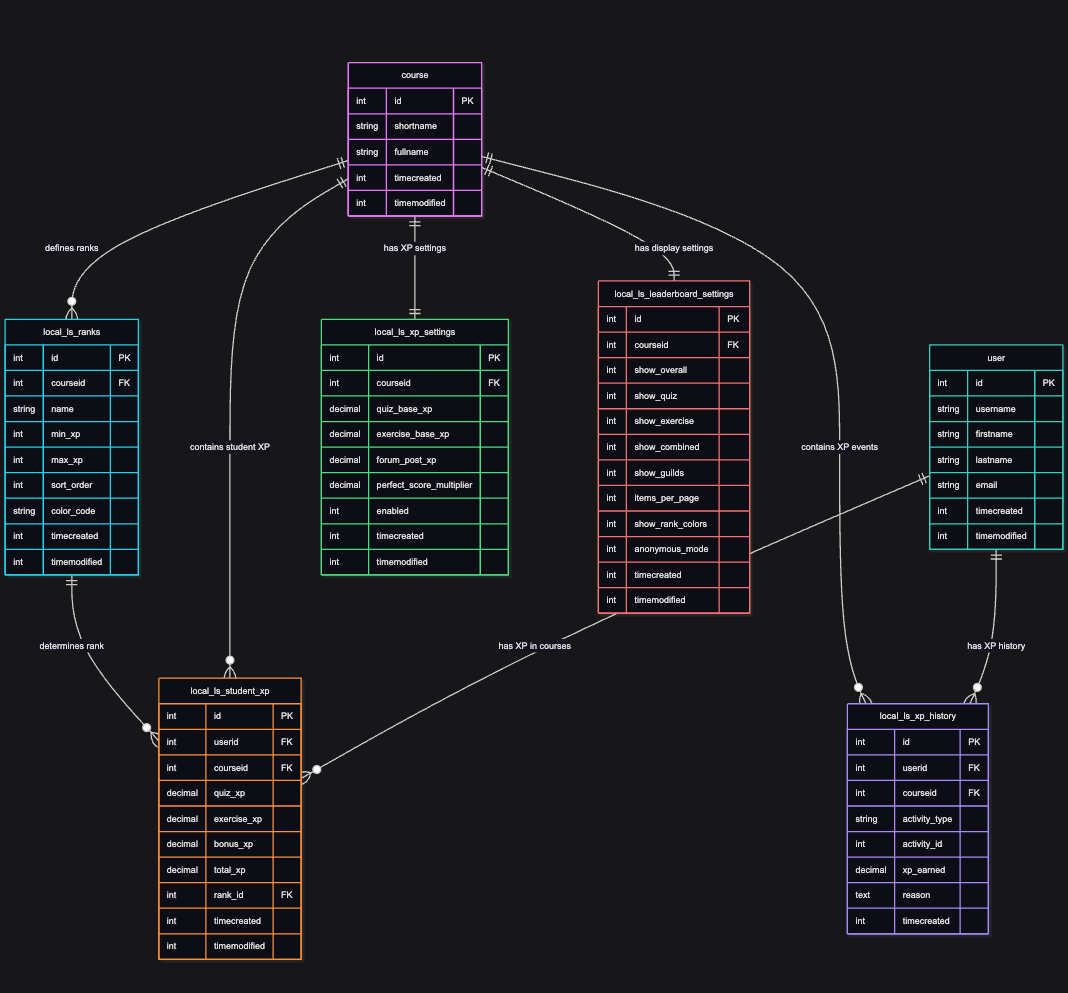
\includegraphics[width=0.8\textwidth]{images/db-er.png}
      \caption{Entity Relations diagram (course is a moodle table shortened for context)}
      \label{fig:db-er-ls}
\end{figure}

\section{Core Features}
\noindent Learning Scorecard 3.0 serves as a proof of feasibility of the system's architecture and thus this iteration will provide the basis of the previous functionality while being extensible to future iterations. At the current state of this dissertation the LS has the folowing core features.

\subsection{Leaderboards}

This iteration of the Learning Scorecard provides five distinct leaderboards:
Overall, Quiz Masters, Exercise Lords, Guild Legends and Combined Champion.
Each present different metrics and calculate the rankings differently.

Overall Leaderboard is the aggregation of all quest XP and calculates the
ranking based on overall course performance.
\begin{figure}[H]
      \centering
      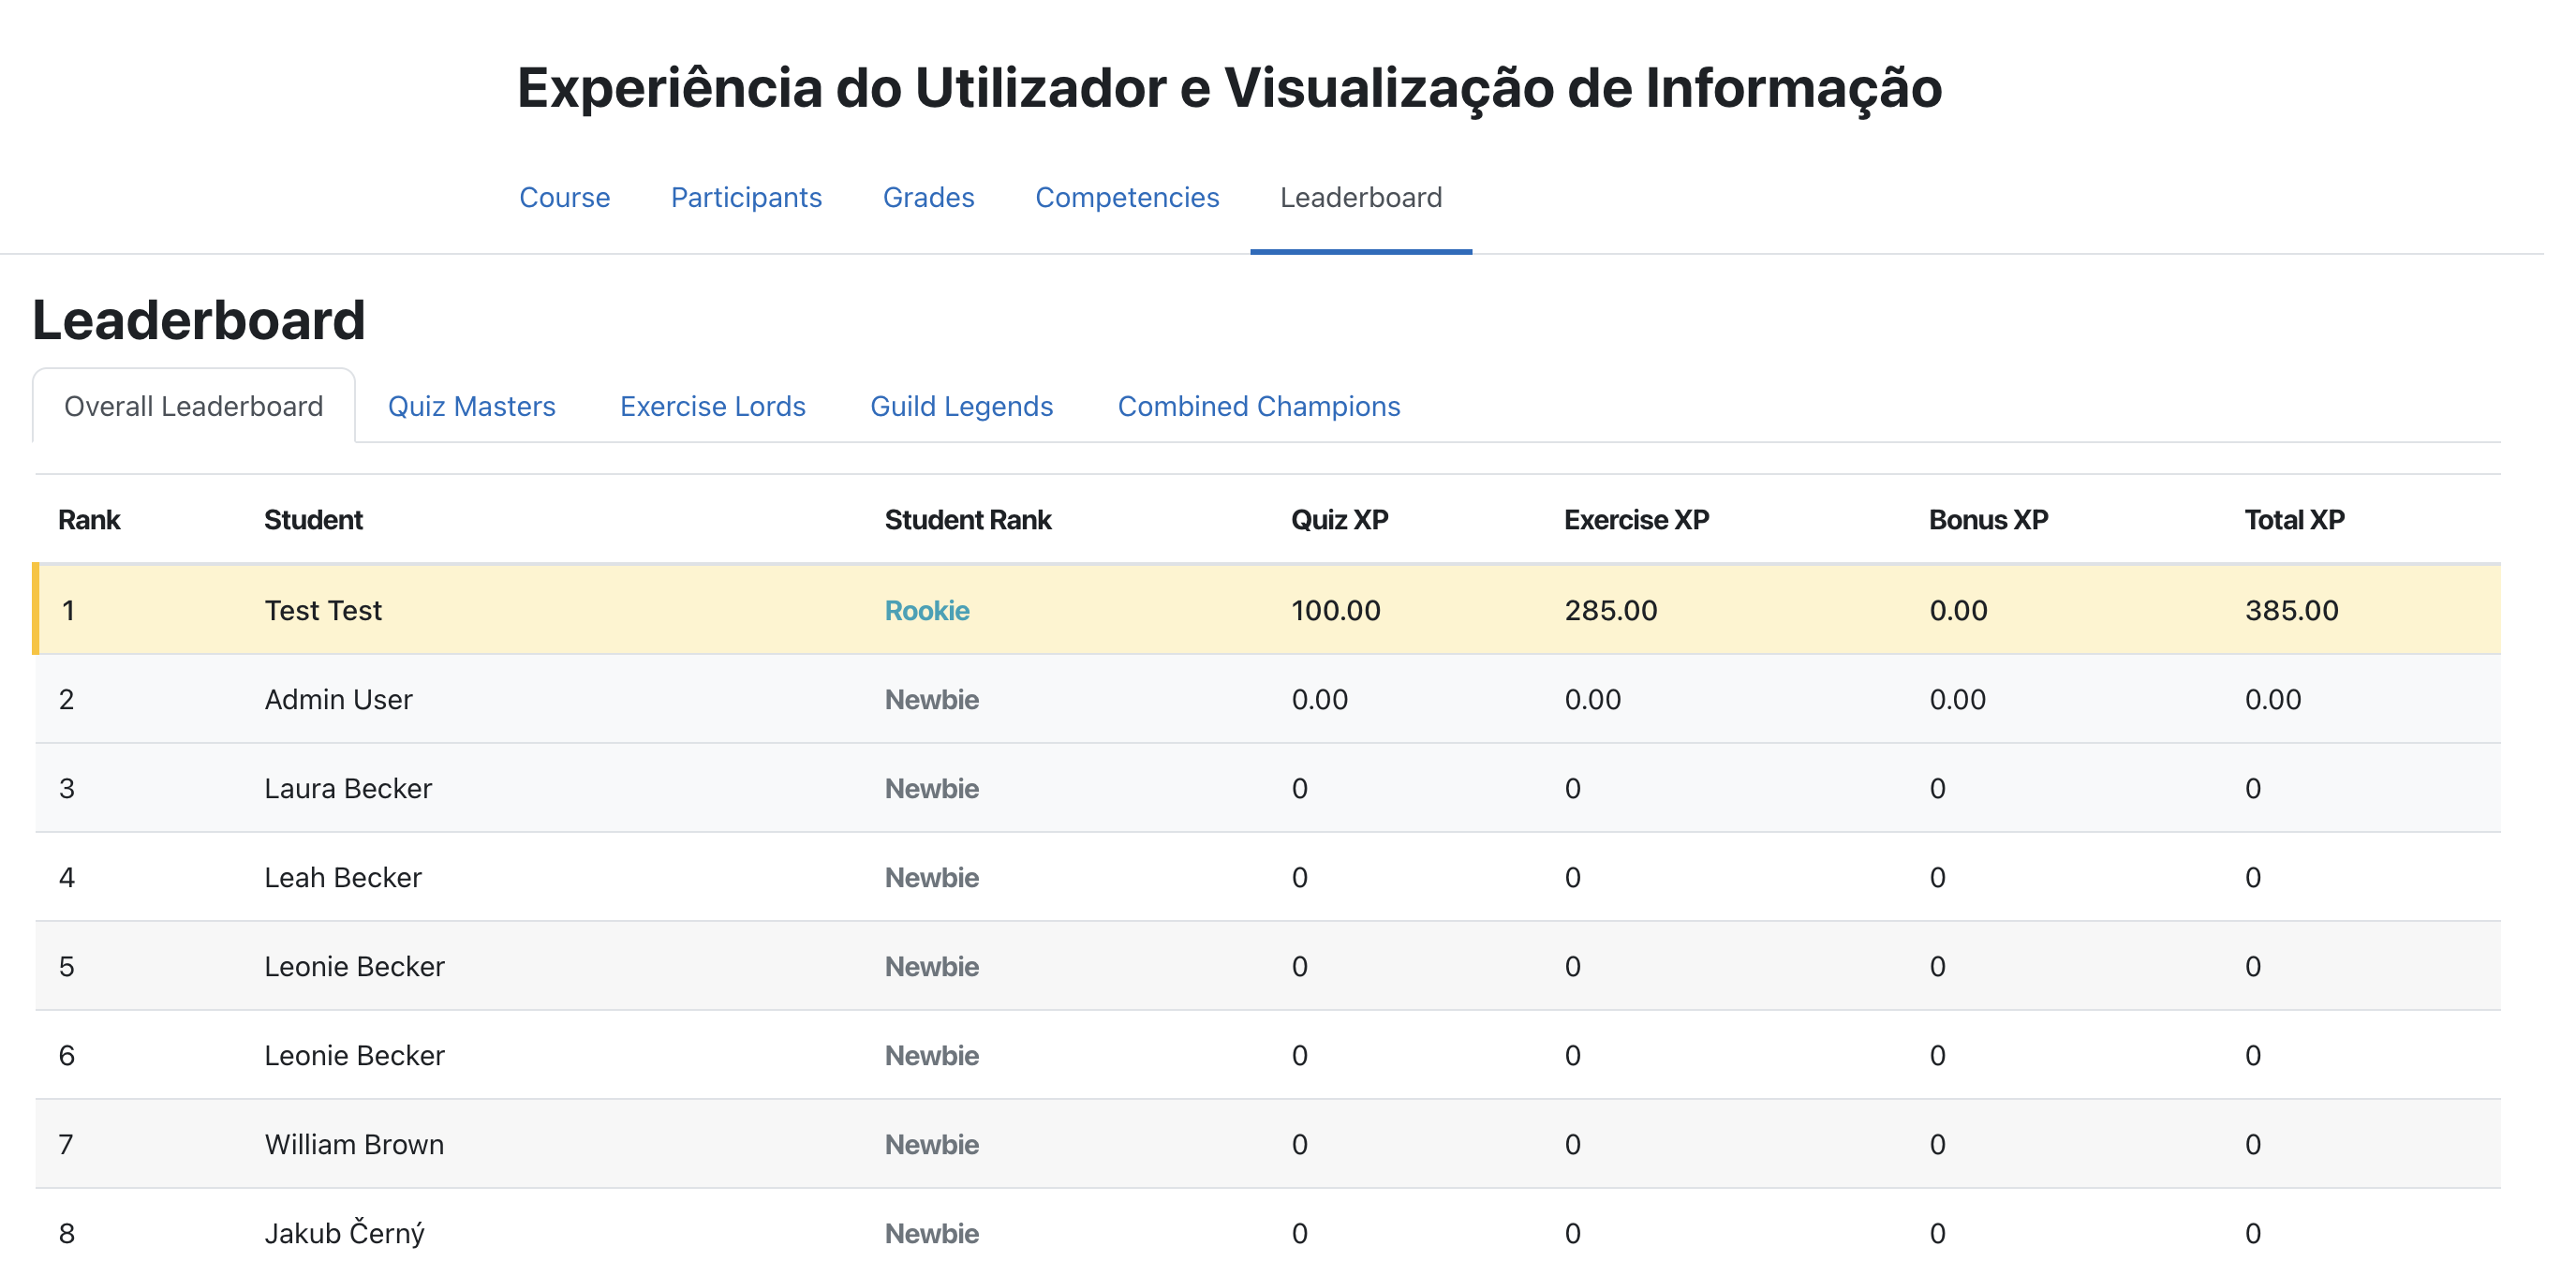
\includegraphics[width=0.8\textwidth]{images/overall-leaderboard.png}
      \caption{Overall Leaderboard Interface}
      \label{fig:overall-leaderboard}
\end{figure}
Quiz Masters focuses on the quiz quest XP and the rankings are calculated based
on it and bonus XP, experience points that are the multiplication of the grade
by the score multiplier defined in the courses LS settings.
\begin{figure}[H]
      \centering
      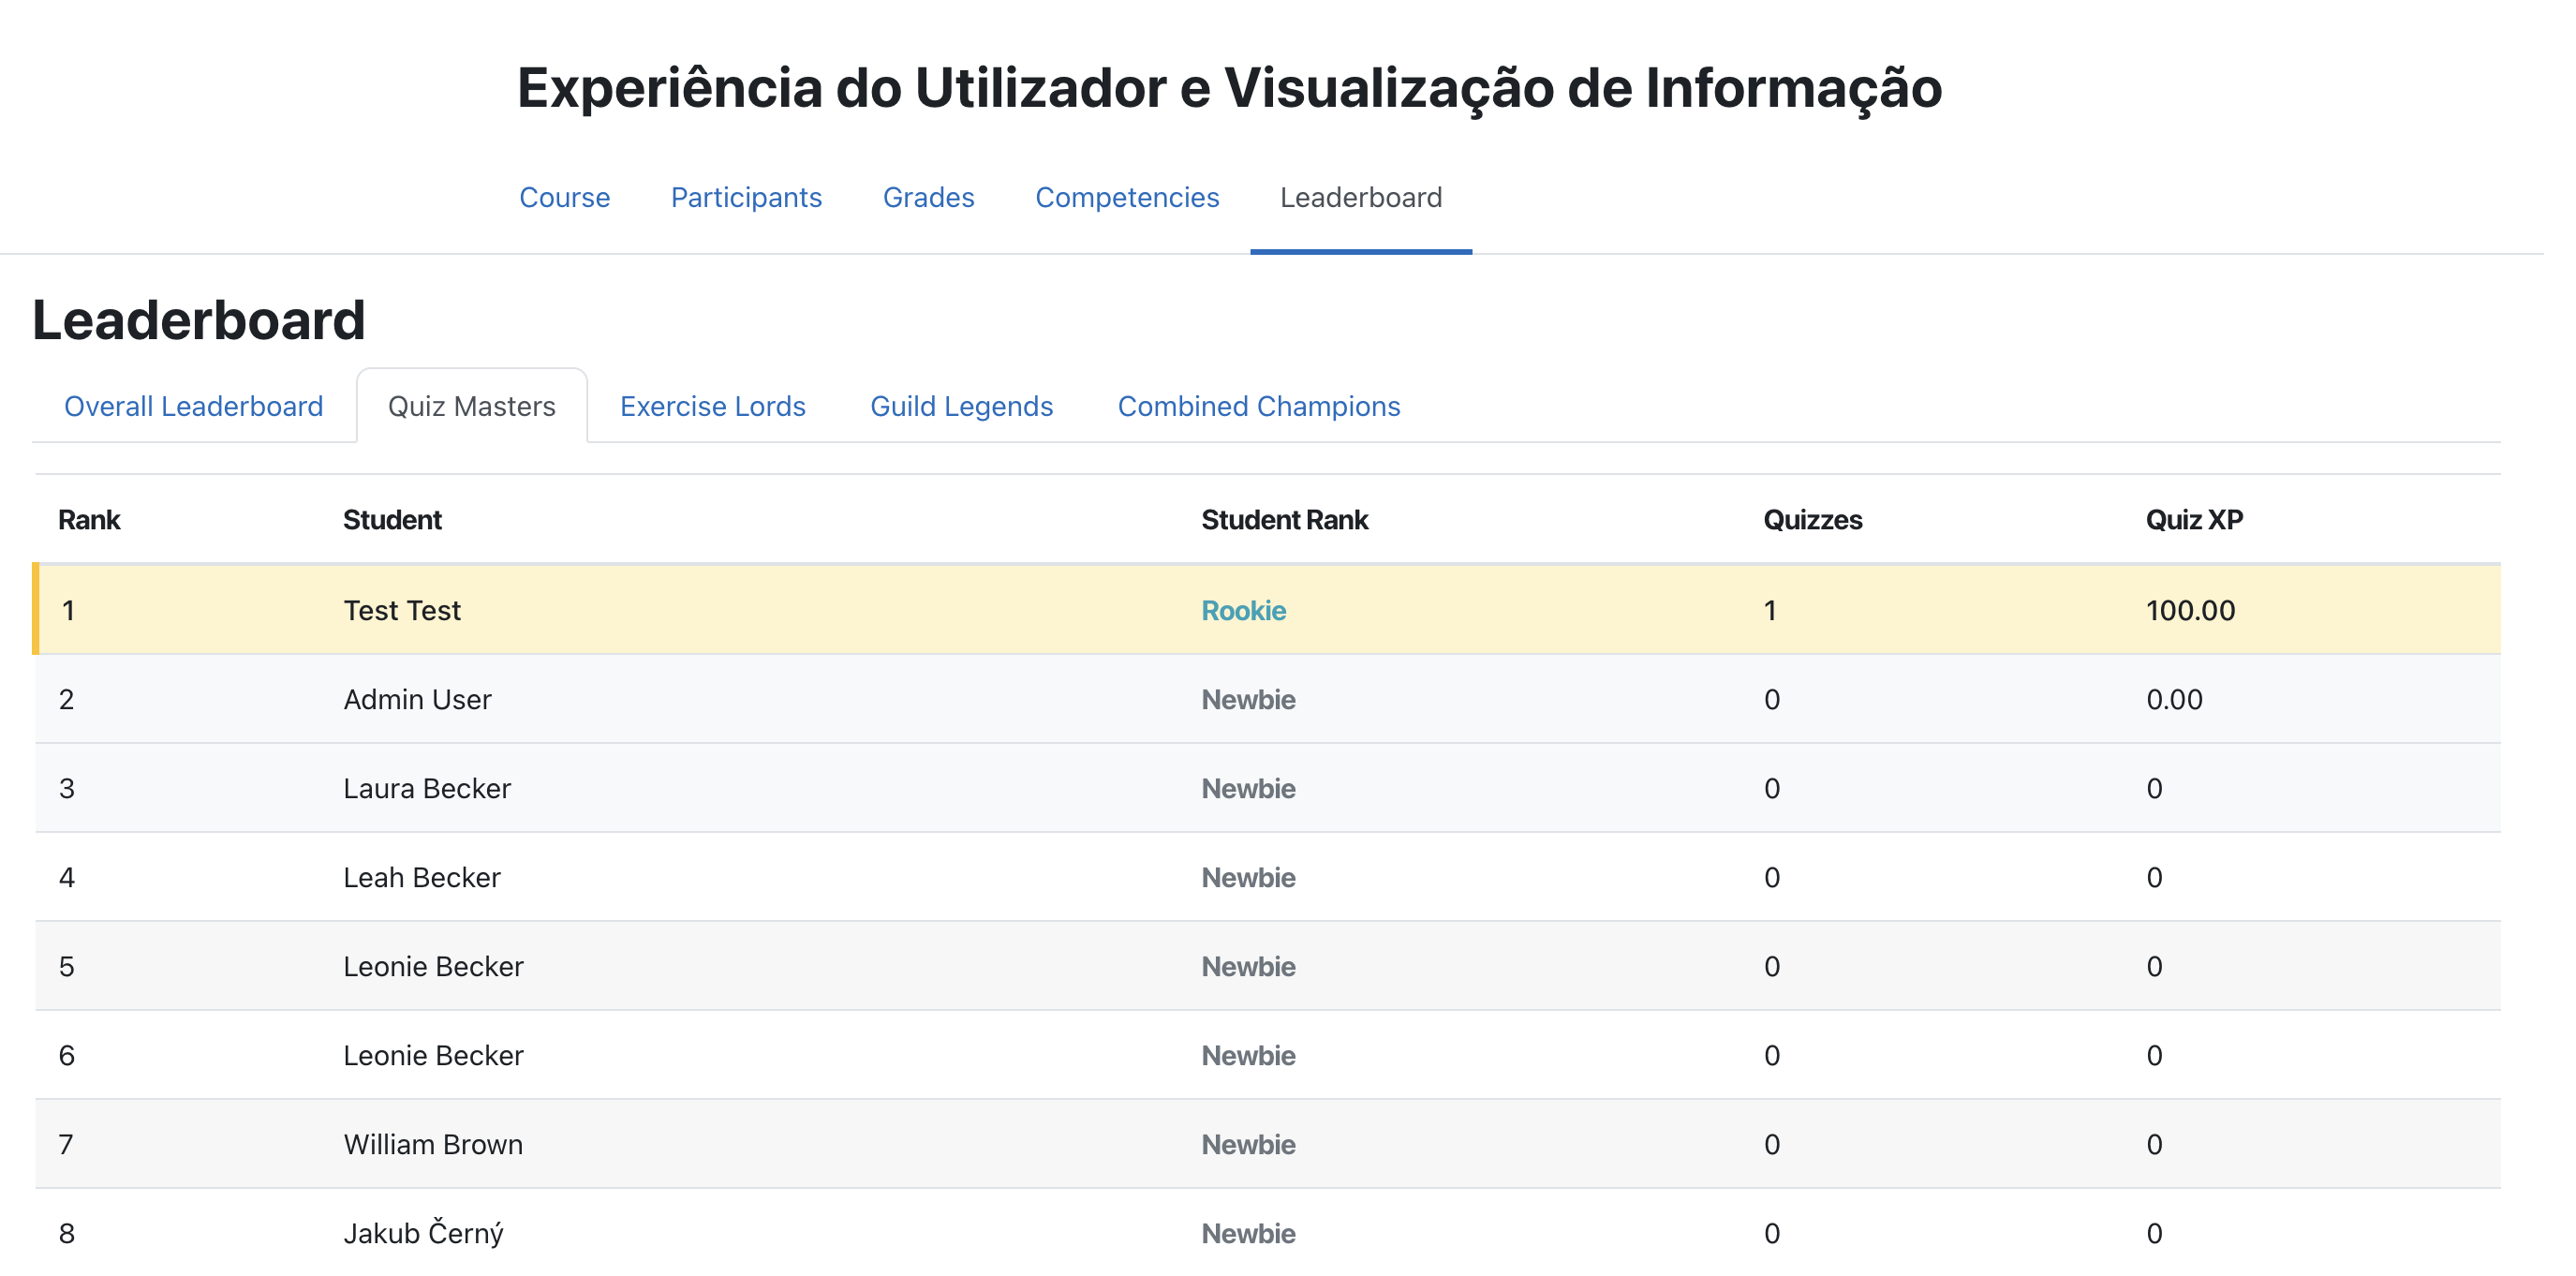
\includegraphics[width=0.8\textwidth]{images/quiz-leaderboard.png}
      \caption{\textit{Quiz Masters} Leaderboard Interface}
      \label{fig:quiz-leaderboard}
\end{figure}
Exercise Lords follows the same formula, exercise quest XP plus the product of
the grade by the score multiplier.
\begin{figure}[H]
      \centering
      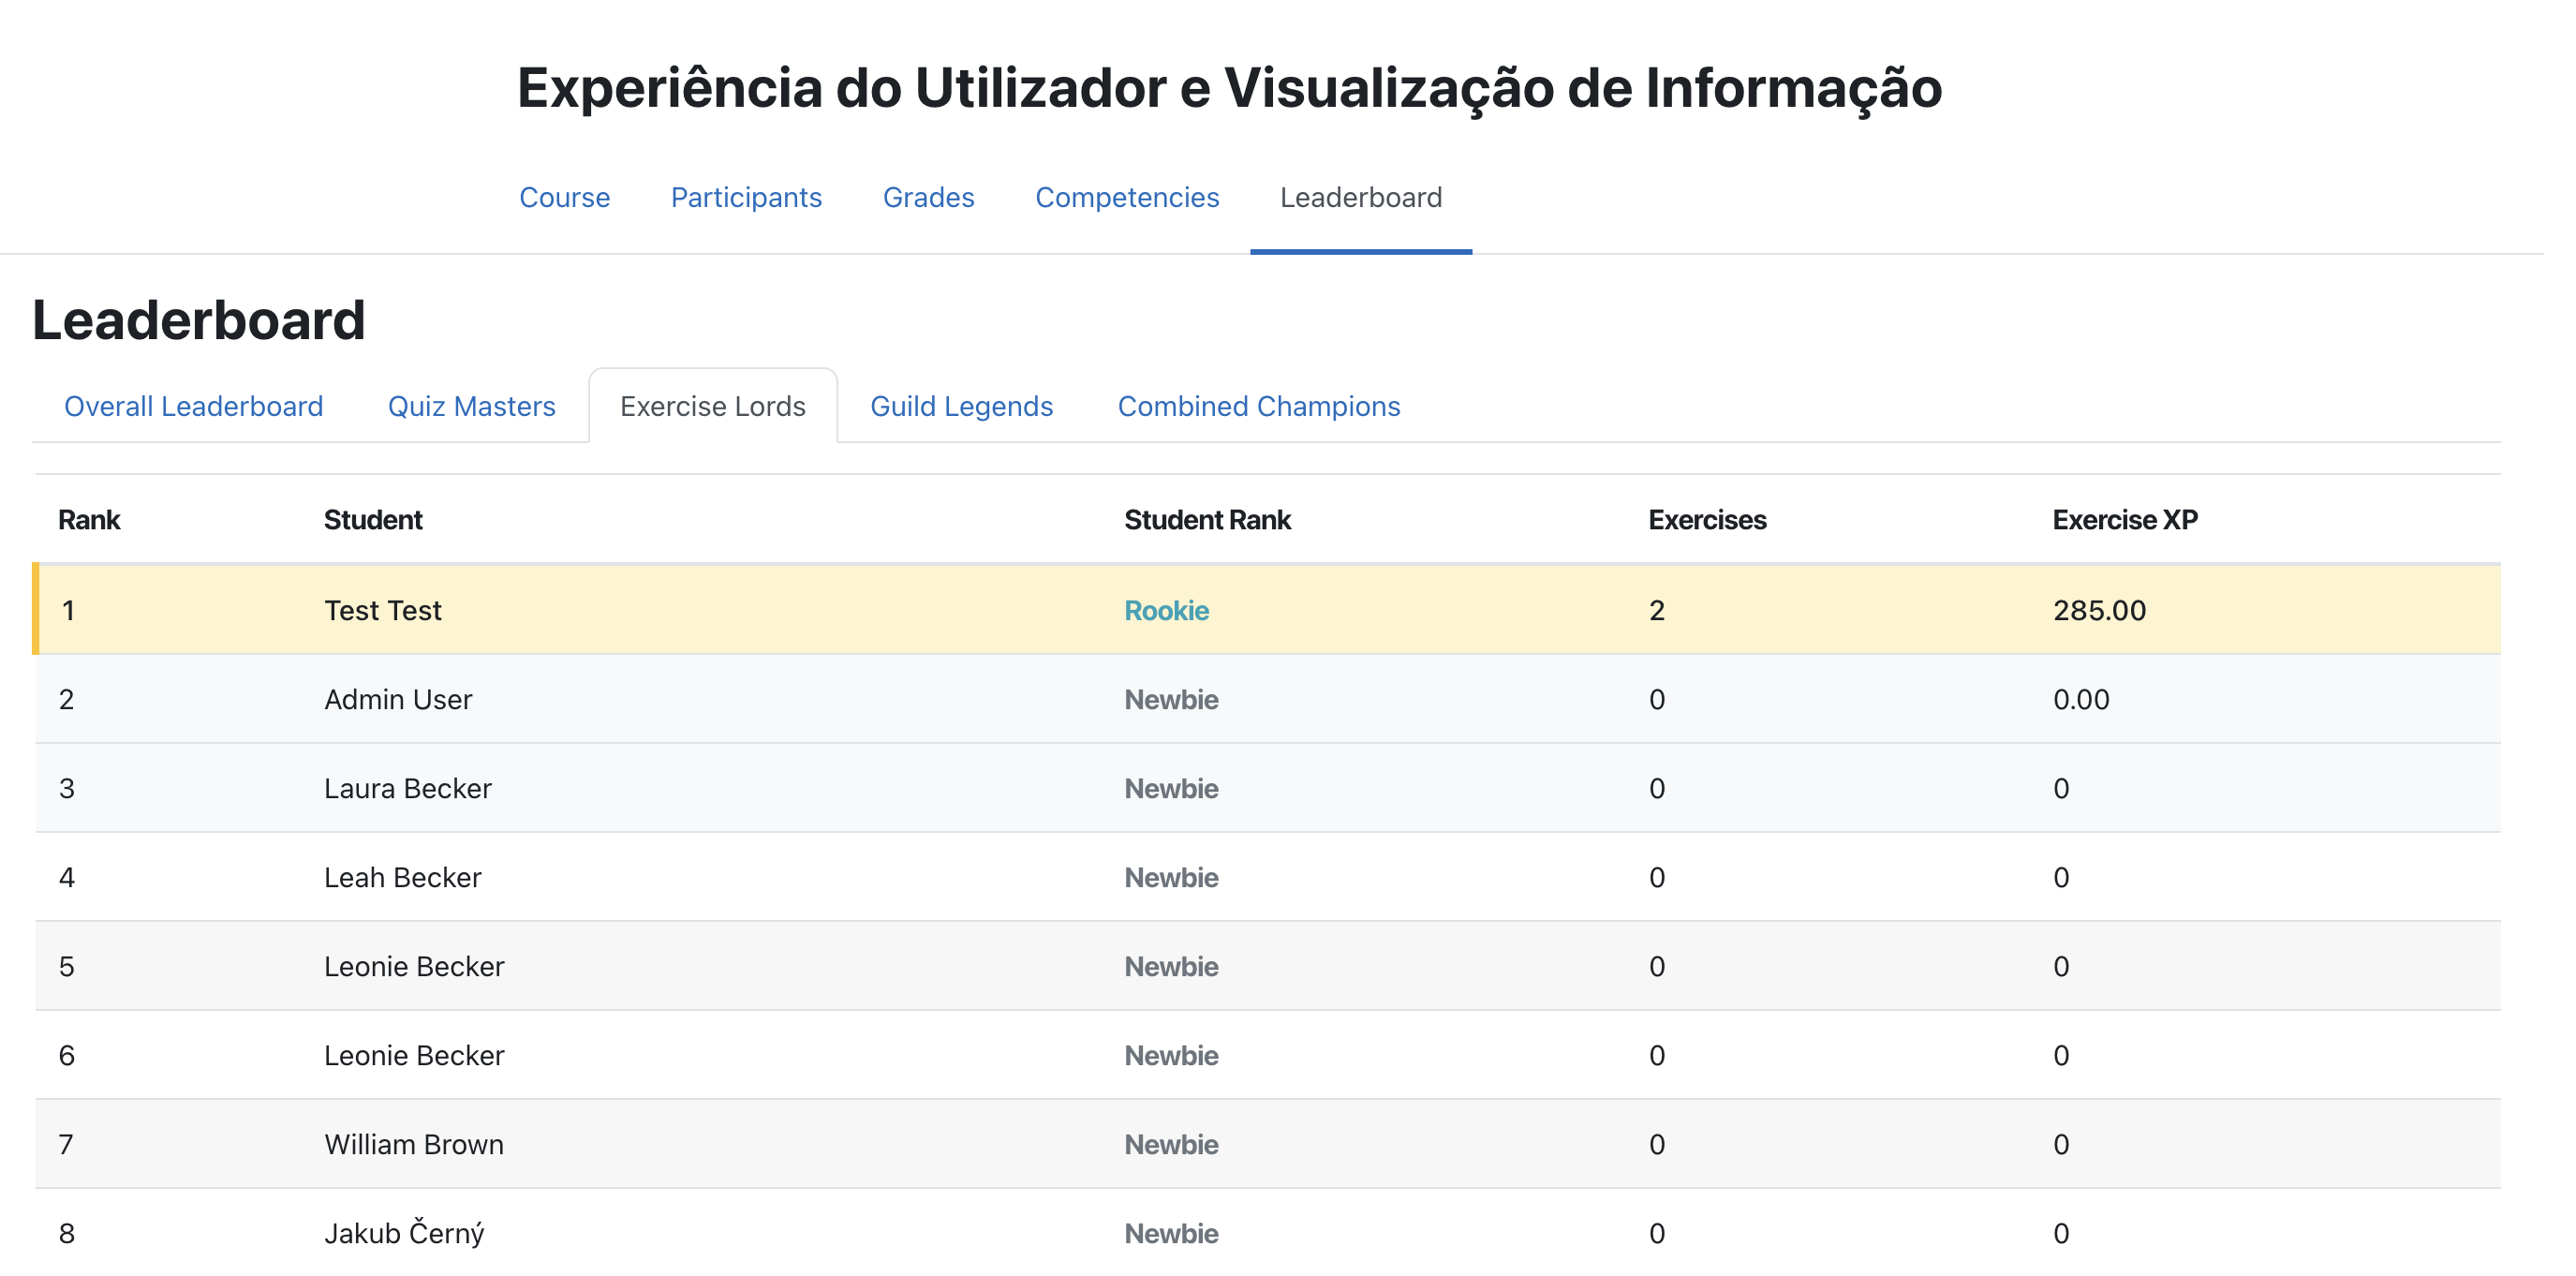
\includegraphics[width=0.8\textwidth]{images/exercise-leaderboard.png}
      \caption{\textit{Exercise Lords} Leaderboard Interface}
      \label{fig:exercise-leaderboard}
\end{figure}
Guild Legends is a leaderboard for the guilds, all members of the guilds
contribute equally for the guild's ranking in this leaderboard. It is achieved through the Moodle's native groups that the teacher or faculty can create.
\begin{figure}[H]
      \centering
      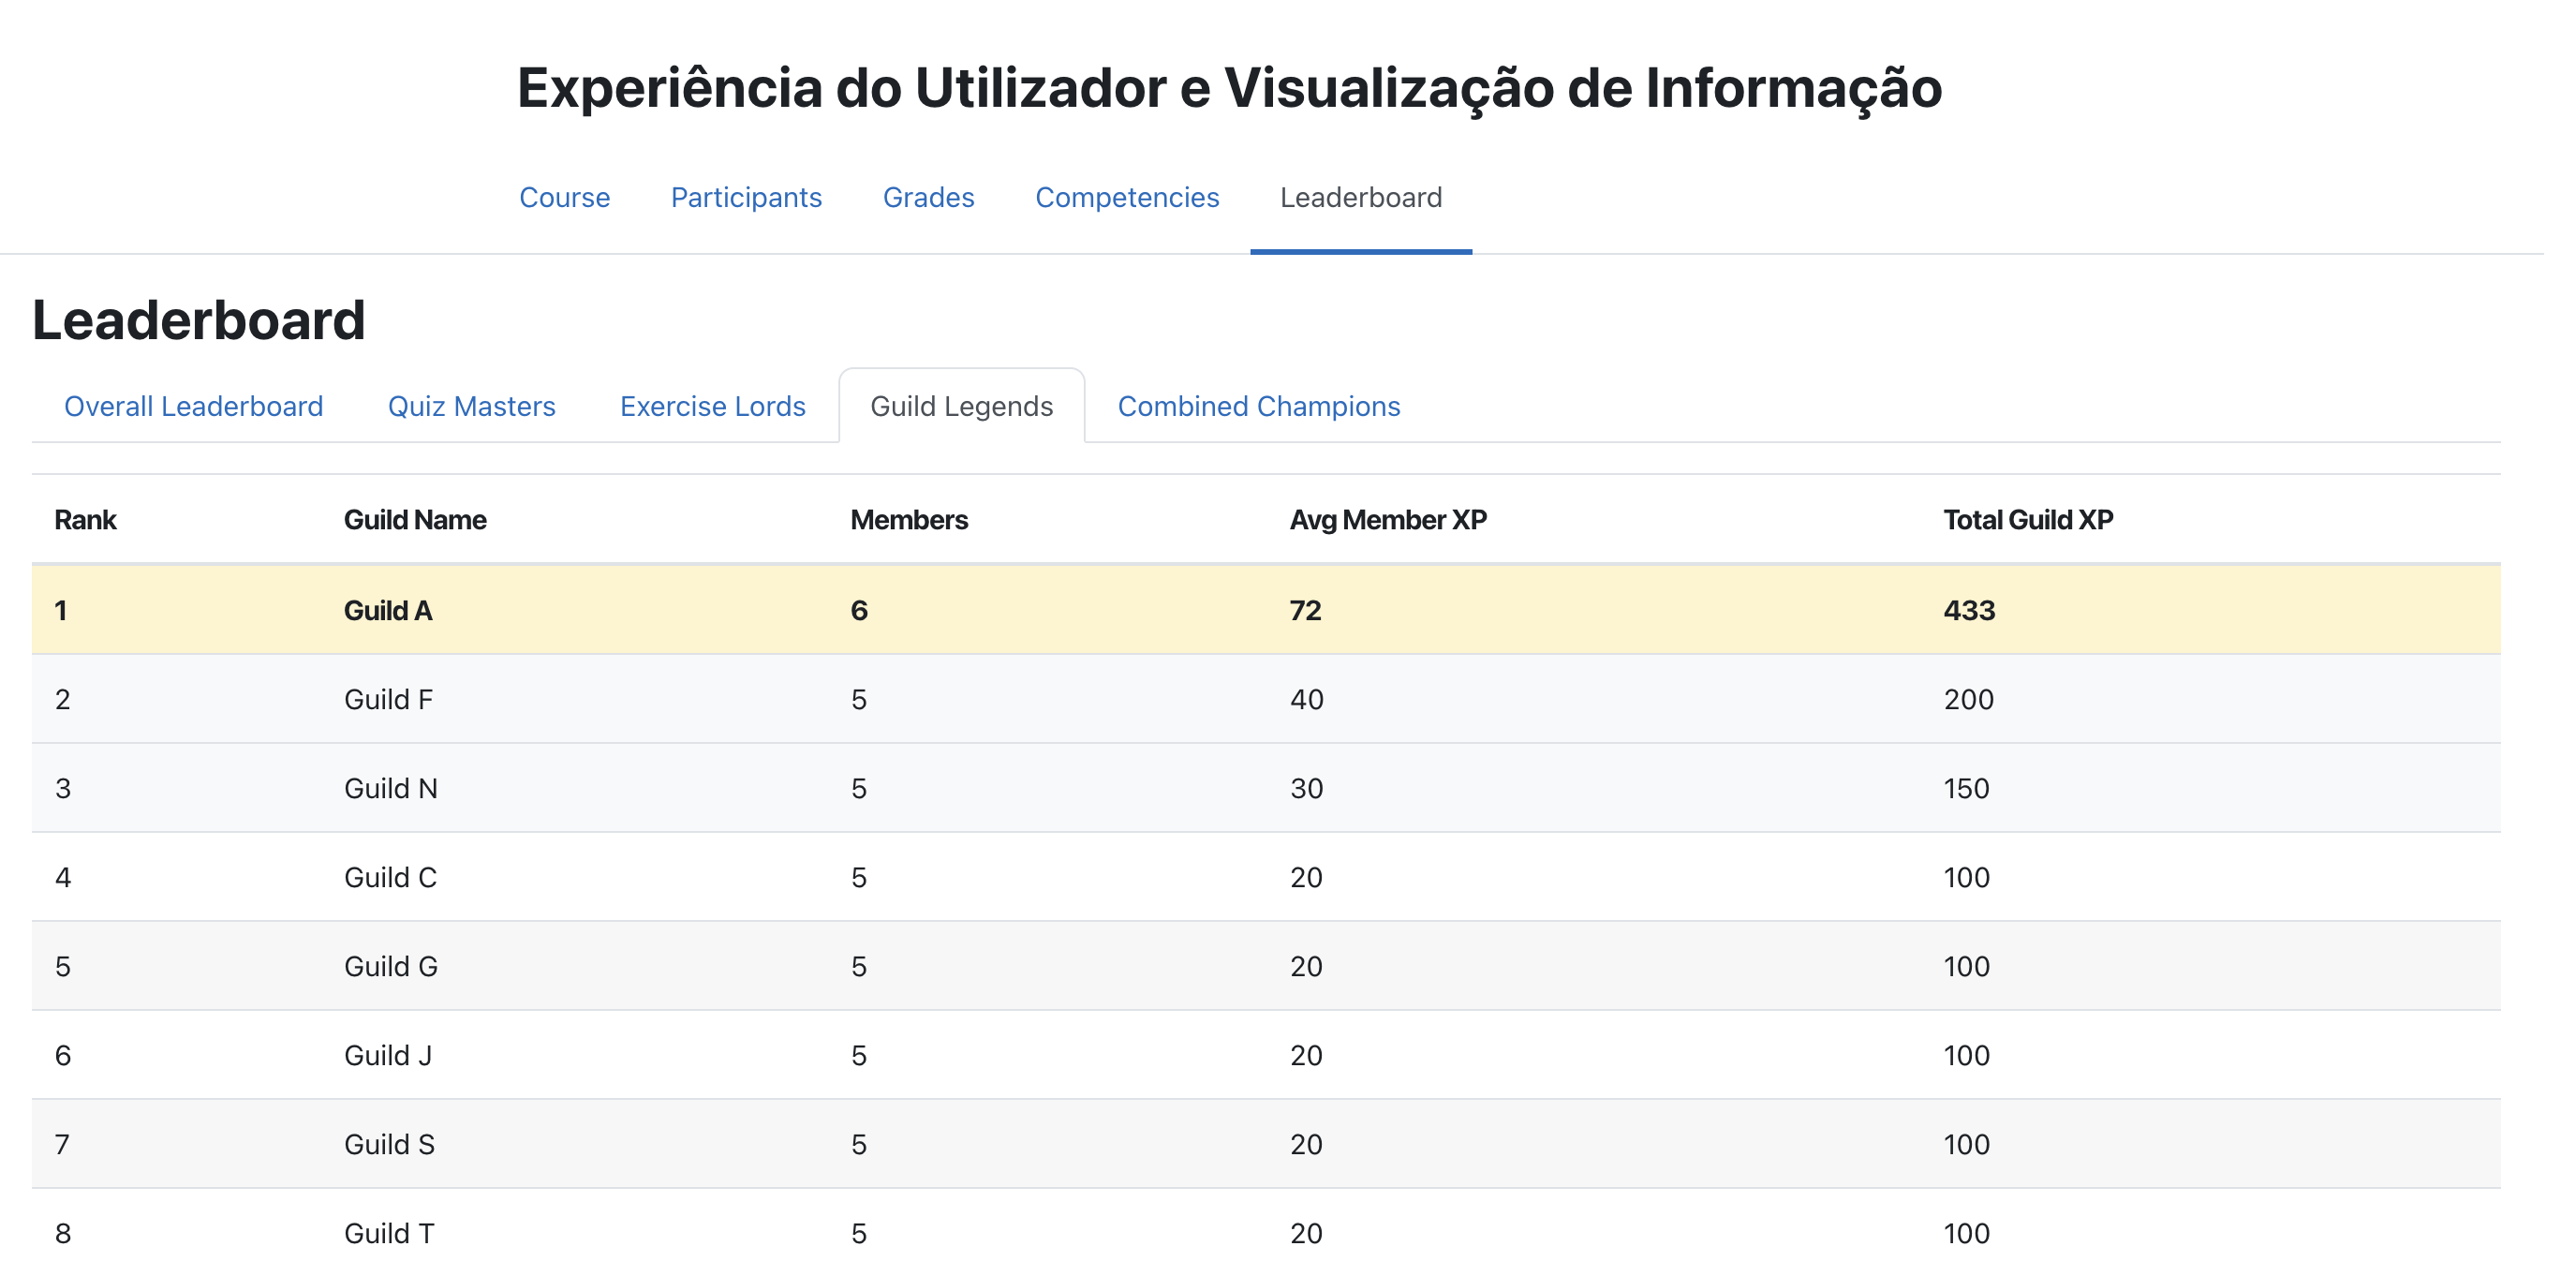
\includegraphics[width=0.8\textwidth]{images/guild-leaderboard.png}
      \caption{\textit{Guild Legends} Leaderboard Interface}
      \label{fig:guild-leaderboard}
\end{figure}
Combined Champion's rankings are calculated by the accumulation of all other
guild's (except for the Guild Legends) leaderboard positions. The student with
the highest rankings on average will be ranked first in it.
\begin{figure}[H]
      \centering
      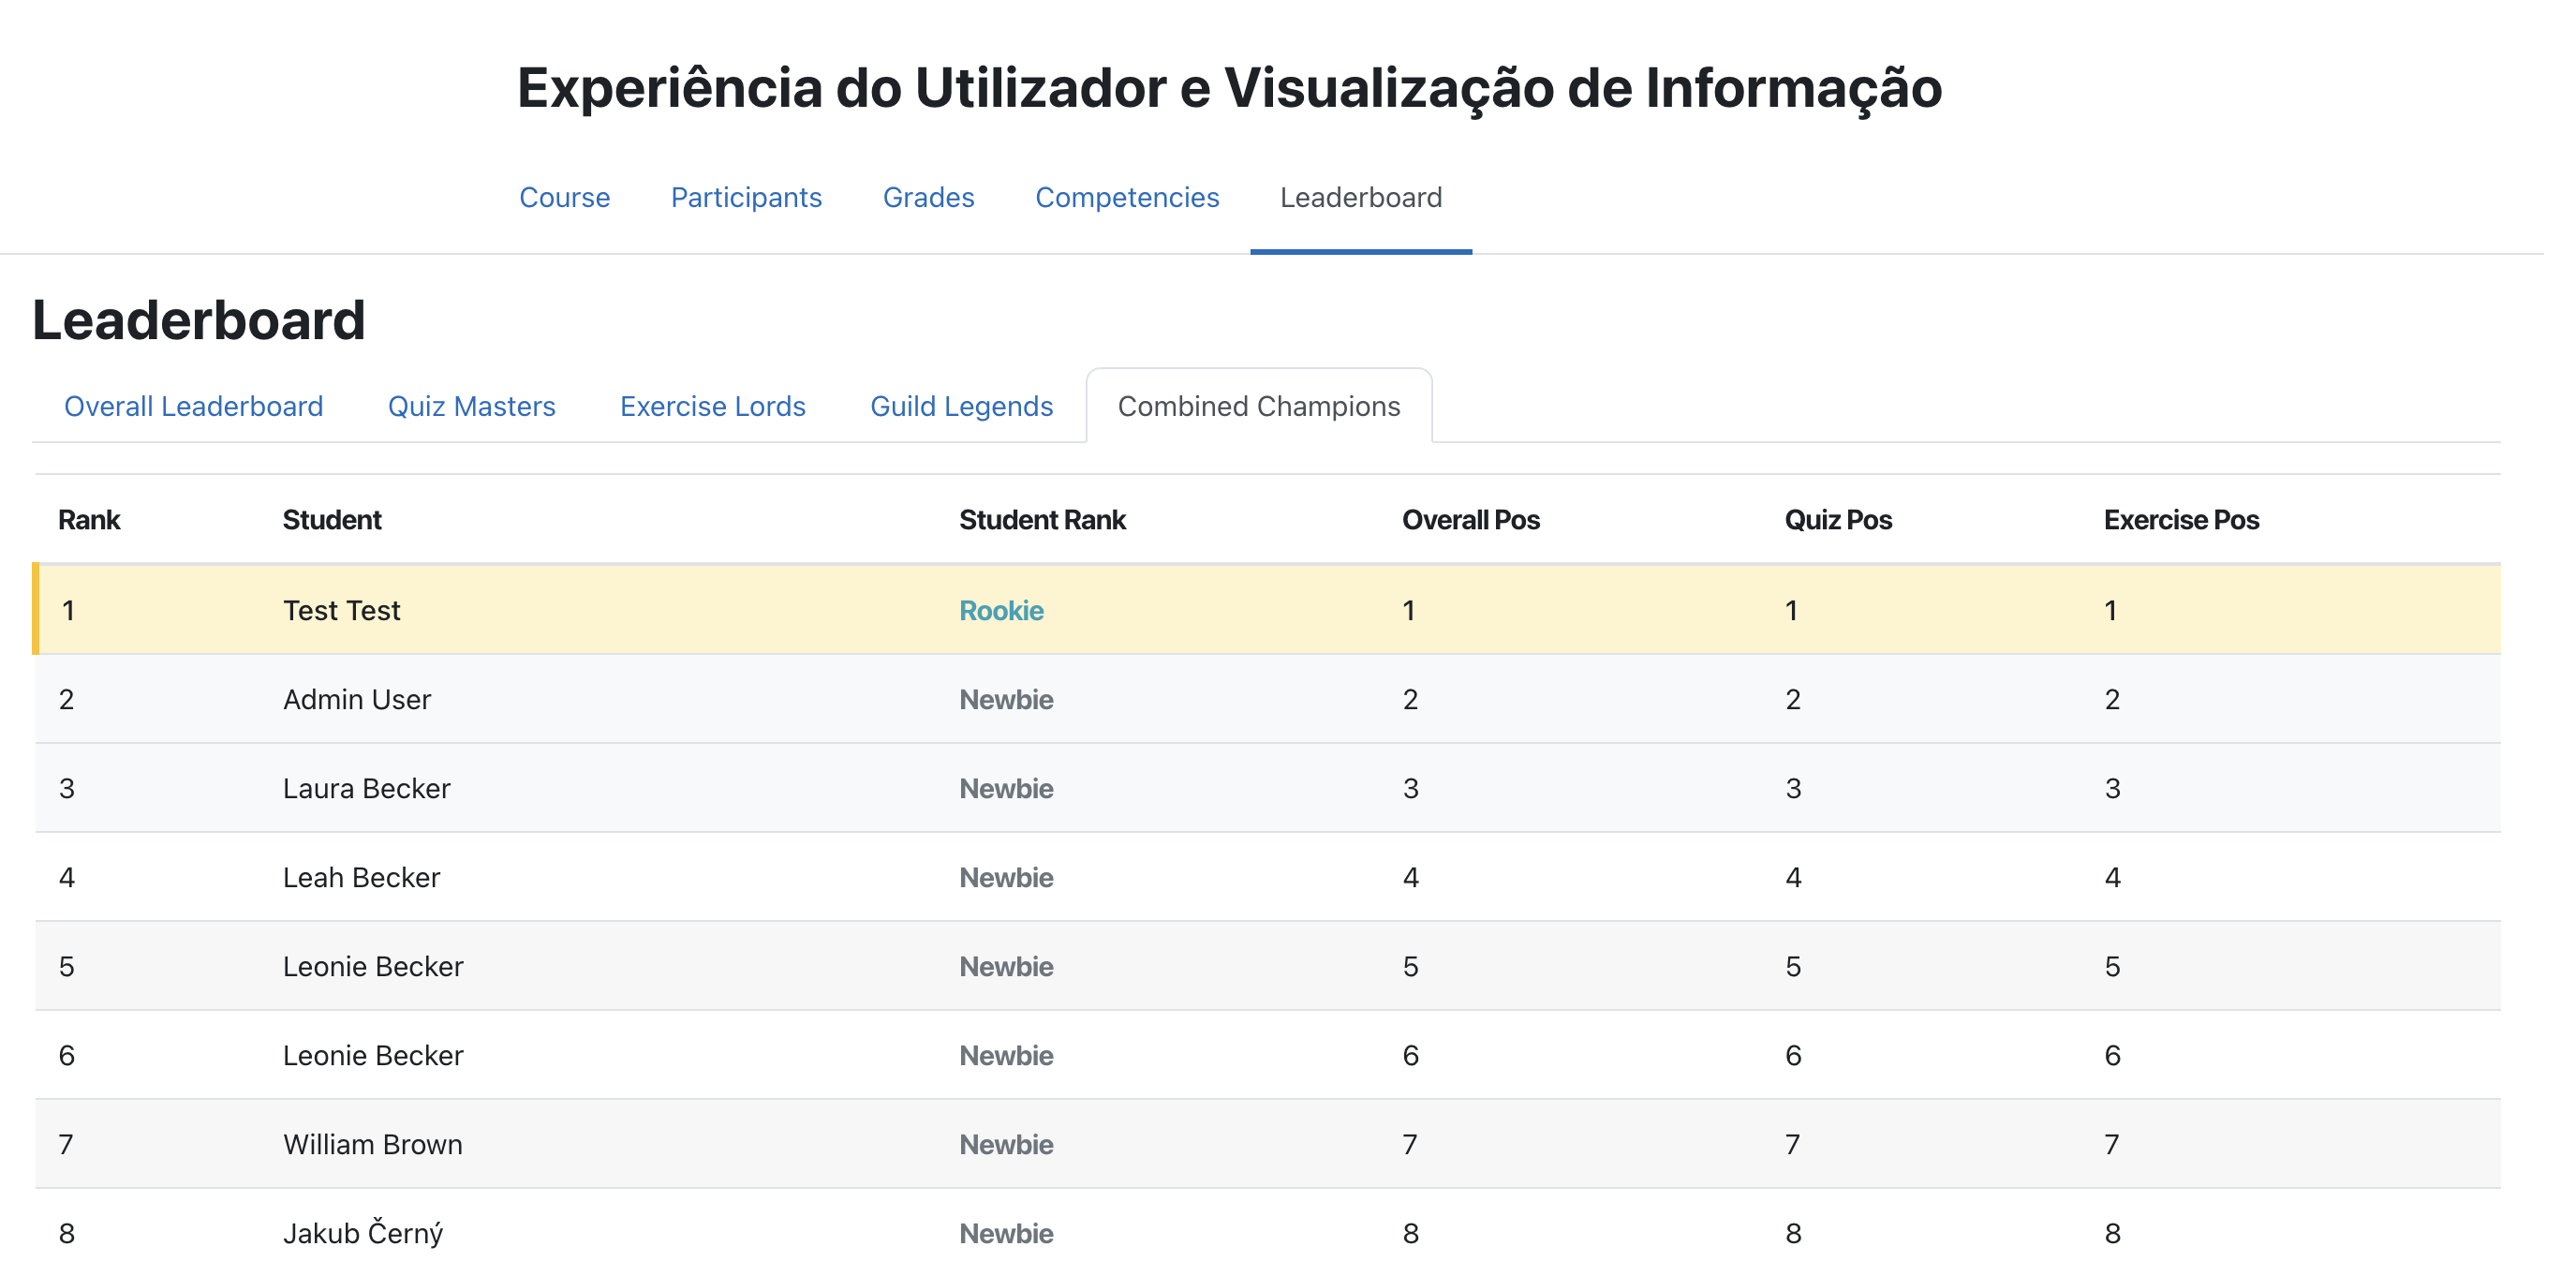
\includegraphics[width=0.8\textwidth]{images/combined-leaderboard.png}
      \caption{\textit{Combined Champions} Leaderboard Interface}
      \label{fig:combined-leaderboard}
\end{figure}

These leaderboards have dynamic ranking, meaning that the positions are
calculated in real-time, providing the most accurate and actual results for the
students. Displayed, there is the position in the leaderboard, the student's
name and the student's rank, except for the guild leaderboard where a guild
name is preferred.

The user interfaces are built using Moodle's native tab navigation for seamless
integration and styling consistency, maintaining the classic Moodle look
without appearing out of place in the course page.

\subsection{Learning Scorecard Settings}

The Learning Scorecard settings page provides an administrative interface for
teachers and faculty to customize the gamification parameters of the course.
This configuration system allows fine-grained control over how students earn
experience points, ranks and of the LS interfaces.

The settings page is only accessible to user with course management
capabilities, ensuring that only teachers and faculty can modify the LS
parameters. The page integrates with Moodle's security framework through
session key validation and capability checks. The settings are also
contextually aware and only apply to the course they is accessed in.

Present in this page are a total of three major sections that can be modified:
(1) The experience points (XP) settings are where the base XP for different
activities and the grade multiplier can be modified; (2) The student rank
configuration defines the rank names, color, thresholds and where the teacher
can also create or remove ranks. (3) The Leaderboard display settings that
customizes how the leaderboards are displayed to the students, has properties
to toggle the visibility of the different leaderboards, insert pagination,
display the rank colours and an anonymous mode that hides the student names.

\begin{figure}[H]
      \centering
      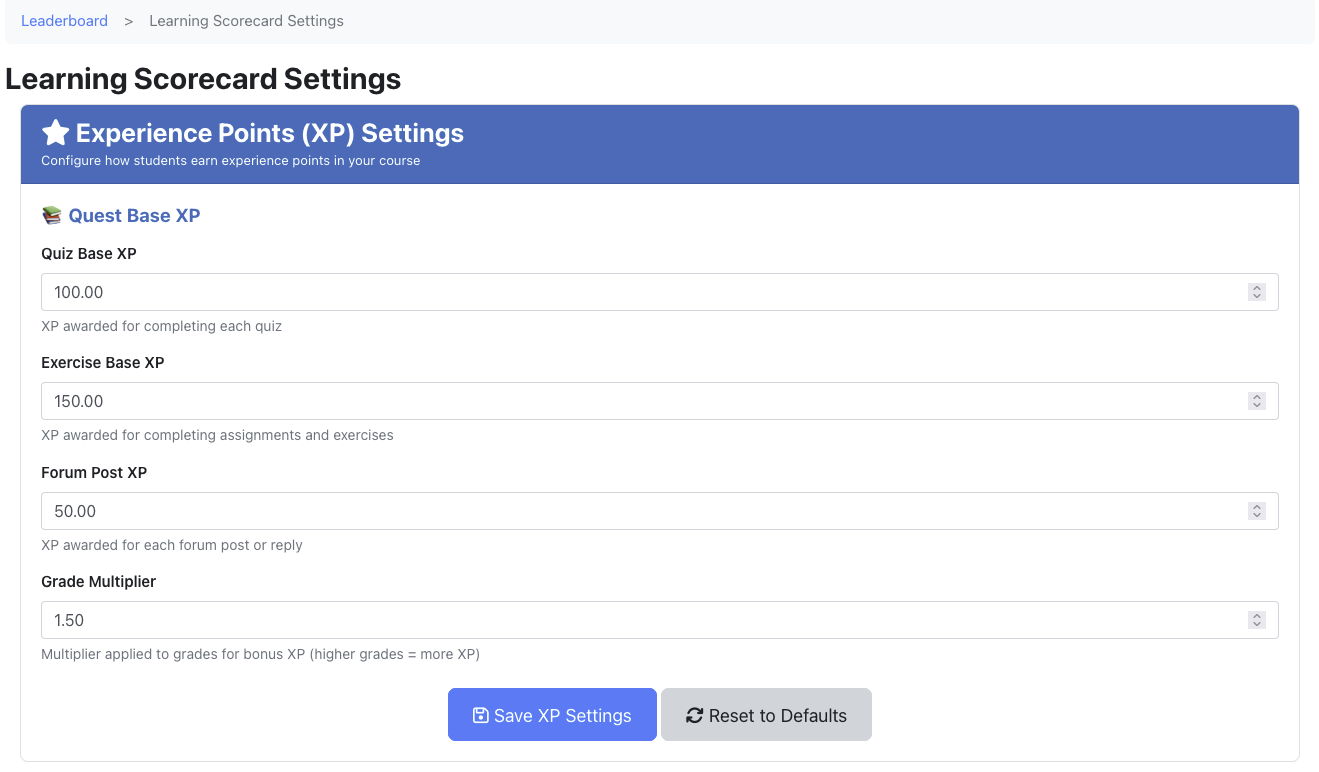
\includegraphics[width=0.8\textwidth]{images/xp-settings.png}
      \caption{XP Settings Interface}
      \label{fig:xp-settings}
\end{figure}
\begin{figure}[H]
      \centering
      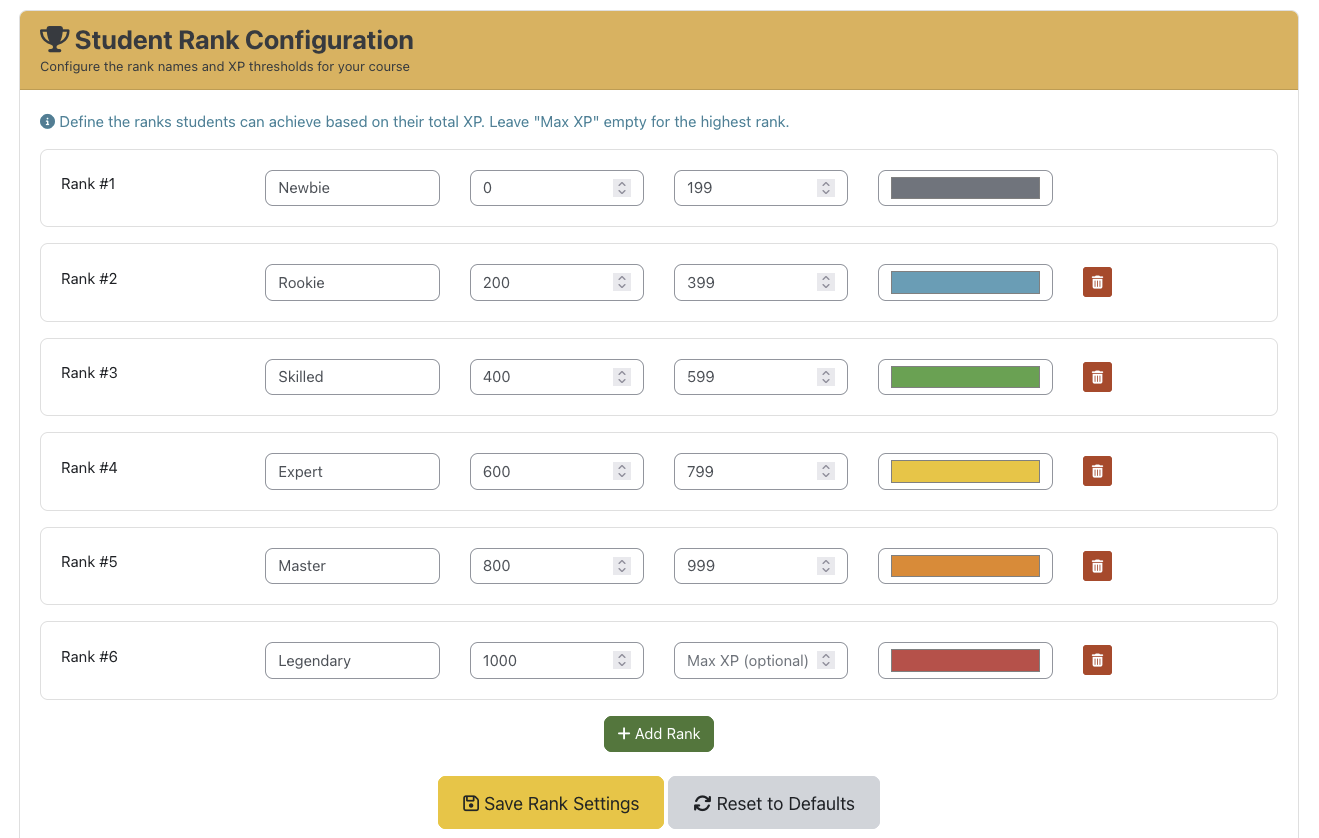
\includegraphics[width=0.8\textwidth]{images/rank-settings.png}
      \caption{Rank Settings Interface}
      \label{fig:rank-settings}
\end{figure}
\begin{figure}[H]
      \centering
      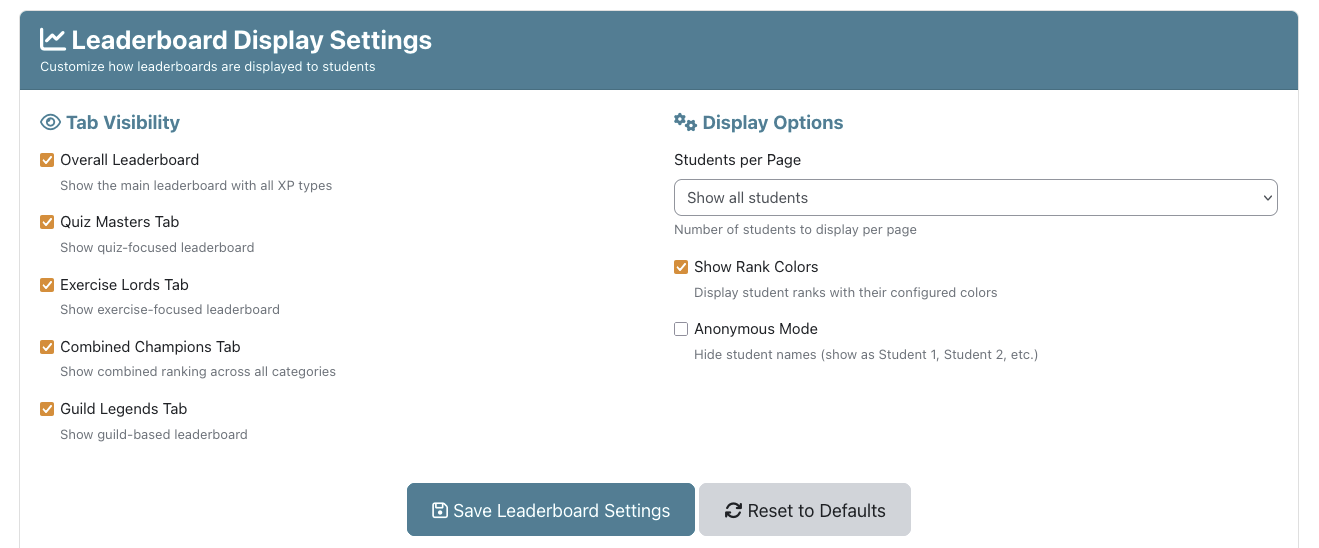
\includegraphics[width=0.8\textwidth]{images/leaderboard-settings.png}
      \caption{Leaderboard Settings Interface}
      \label{fig:leaderboard-settings}
\end{figure}

In this page there is also a section for the badge management that is left
there as a placeholder for future work and improvements.
\begin{figure}[H]
      \centering
      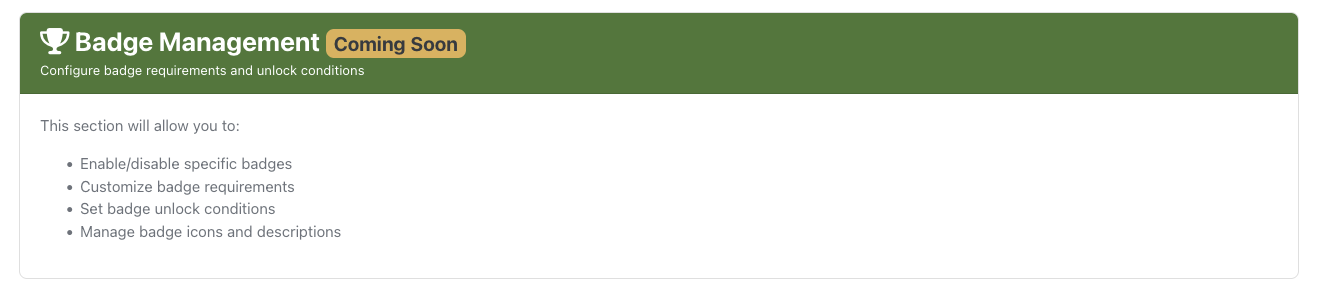
\includegraphics[width=0.8\textwidth]{images/badge-management.png}
      \caption{Badge Management Interface Placeholder}
      \label{fig:badge-management}
\end{figure}

\subsection{Experience Points (XP) and Ranking System}

Present in this iteration is also a XP System that provides real-time XP
calculation through event observers that trigger upon quiz completion and
activity submission. Grade based XP multipliers and perfect score bonuses are
also applied to every quest completed by the students.

The LS 3.0 provides an XP configuration system that allows per-course settings
with customizable base XP values for different activity types, configurable
grade bonus and an audit trail through an XP history table that logs every XP
transaction. All XP settings are stored in the moodle database natively with
fallback default values and automatic creation upon course initialization.

All XP accumulated by each student maps into a 6 tier ranking system that
follows the definition found on previous versions: Newbie - Rookie - Skilled -
Expert - Master - Legendary. These rank intervals are all available to be
defined per course in the LS settings page. There are rank badges displaying
both on the dashboard block of each student and on the leaderboards next to
their name. On the dashboard there is also a percentage-based progress bar with
"XP to next rank" indicator.

With the notification system native to Moodle, the LS 3.0 can send a
notification on rankup, in order to provide an extra boost of motivation as it
was designed for in previous iterations of moodle.

\subsection{Dashboard Block Plugin}

The dashboard block plugin was created as a proof of concept of the learning
scorecard previous version's dashboards with graphs and learning metrics. It
was a achieved through a auxiliary plugin created within the moodle
architecture that is only responsible for the UI blocks that the students can
insert into the dashboard. There can be a lot of different blocks each with
their defined metrics and graphs for a rich visualization interface of the
students' learning performance.

The current and only block present in this plugin is a visualization of the
student's rank (see Figure \ref{fig:block-plugin}), progress to the next rank
with a percentage-based progress bar and a breakdown of all XP earned. There is
also an ability to cycle through multiple courses and display the XP for the
course selected.

\begin{figure}[H]
      \centering
      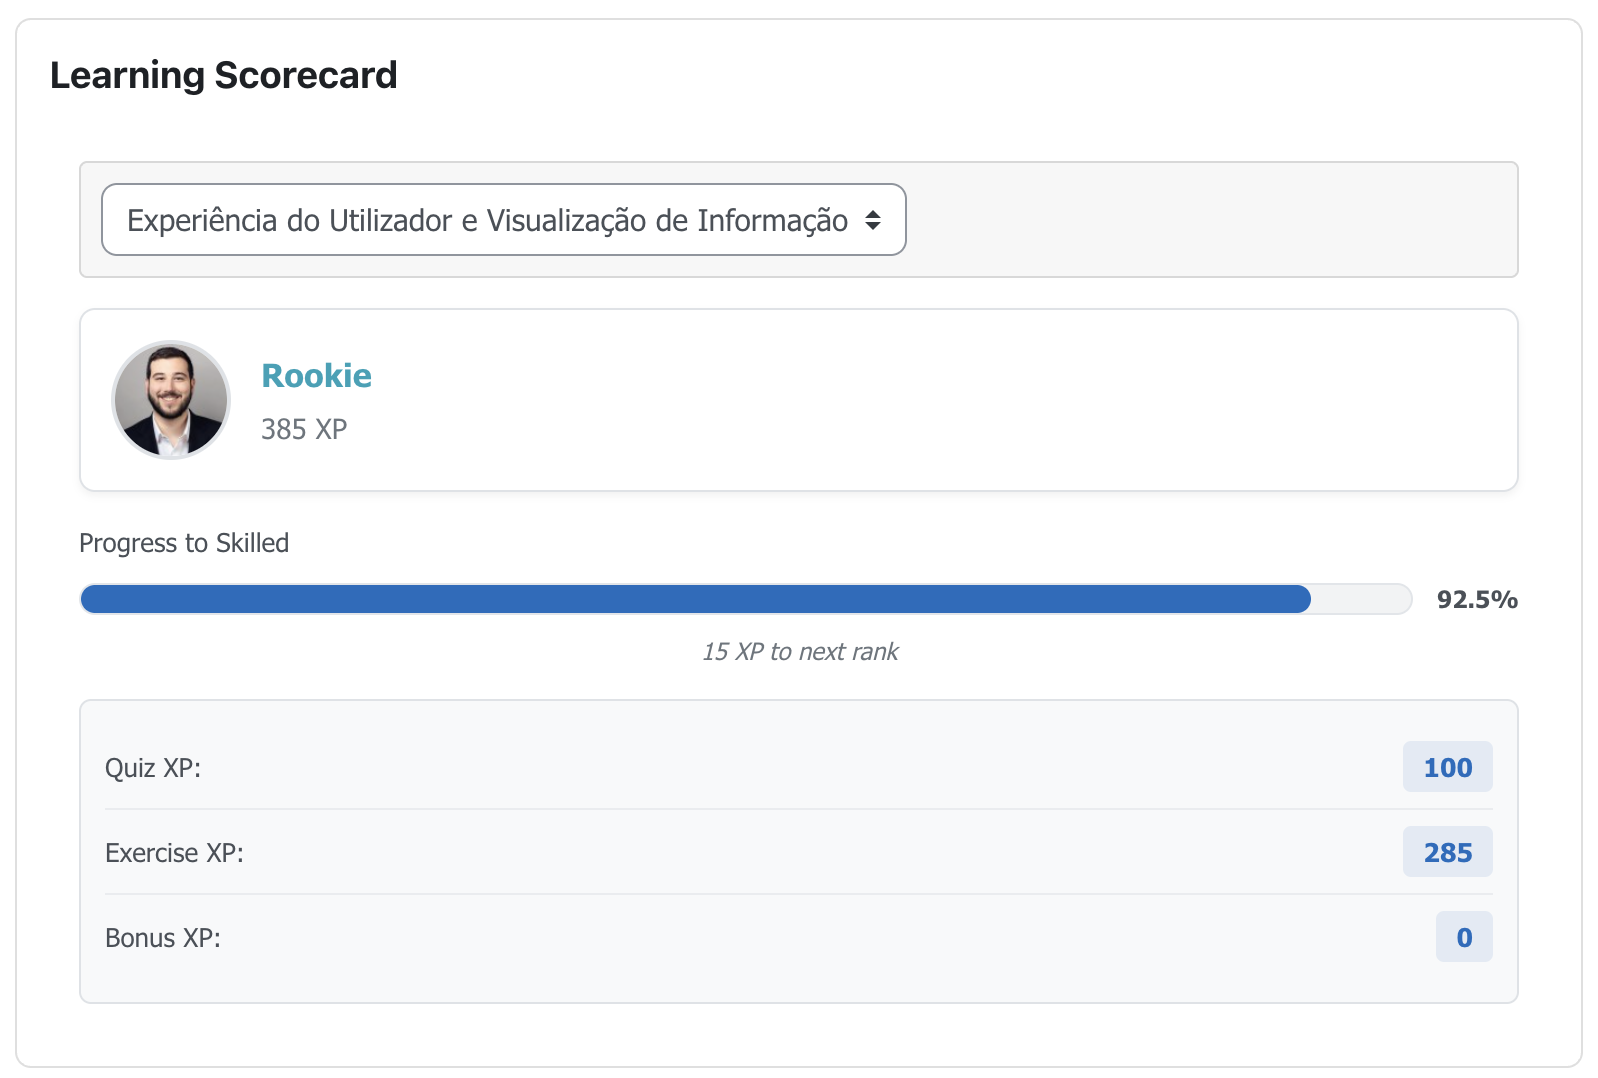
\includegraphics[width=0.8\textwidth]{images/block-plugin.png}
      \caption{Dashboard block plugin student XP Interface}
      \label{fig:block-plugin}
\end{figure}

All data presented in the block is retrieved through queries to the moodle
database and the tables that were appended through the Learning Scorecard Local
plugin. This allows for a better division of responsibilities of each plugin
and provides a much better and objective architecture that can be easily
extended in the future.

Another topic to address is the language of the interfaces and text. Every
plugin has two language packs, folders in the plugin configuration that provide
translations of text and strings. Currently, the LS 3.0 is able to be
translated into portuguese and english and the language packs are chosen
automatically depending on your moodle's language.

\section{Challenges \& Limitations}
\noindent Throughout the conception and development of the Learning Scorecard 3.0 there were a few challenges that proved difficult to resolve, requiring trade-offs and becoming contraints in the current implementation.

One big challenge from the LS 3.0 is the Moodle environment unapproachibility
and inconsistency. The instance hosted by ISCTE changes versions regularly,
proving to be possibly difficult to maintain and keep the LS 3.0 up to date,
although the plugin architecture presents compatibility with Moodle 4.1+. In
institutional environments with legacy Moodle installations this may limit
deployment flexibility or even force them to abandon integration all together.

The current leaderboard position calculation methodology requires loading
entire student datasets into memory for PHP-based sorting algoriths. This
approach presents some scalability concerns, particularly evident in the
combined leaderboard where multiple leaderboard arrays are maintained
simultaneously. The current implementation could benefit with optimizations in
the pagination and how the leaderboards are loaded and sorted to avoid memory
exhaustion in courses with extensive enrollments. Not only that, the
leaderboard generation system relies heavely on multiple sequential SQL queries
and could be a potential performance bottleneck in high load intensity.

The XP audit trail could accumulate a substantial data volumes over time
without implemented achival strategies. This design decision prioritizes
complete historical data but presents long-term storage scaling challenges and
query performance degradation as data accumulates.

The current database schema maintains a strict per course data separation,
preventing cross-course analytics. While this architectural decision maintains
data privacy, it restricts the potential for comprehensive learning analytics
across multiple courses for both the teacher and the students.

It is imperative, when attempting to mature this proof of concept, to take in
consideration these limitations and tackle the possible chockeholds of the
application.
\chapter{Conclusions}
\noindent~This dissertation has demonstrated success transformation of the Learning Scorecard from a standalone web application to a fully integrated Moodle plugin system. Learning Scorecard 3.0, although just a proof of concept, represents a architectural evolution that addresses the critical adoption barriers identified in previous iterations while perserving core gamification capabilities and providing a stable foundation to build features that weren't ported to this version.

Practically, this dissertation delivers a functional proof of concept that
eliminates the authentication hurdles, mnual data entry and infrastructure
maintenance burdens that constrained previous implementations. The plugin-based
architecture sucessfully leverages Moodle's student activity data, role-based
access control and established user workflows to create a seamless integration
and gamified learning experience.

\section{Recommendations for Institutional Use}
\noindent~Higher educational institutions considering Learning Scorecard 3.0 adoption should take in consideration recommendations prior to a broad institutional use. A controlled pilot deployment within academic contexts focusing on courses with moderate enrollment sizes in order to validate system performance and gather ser feedback is critical and imperative to avoid scalability bottlenecks.

Technical infrastructure should be ensured by institutions in a way that
alignes with the system requriements of the LS 3.0, including Moodle version
compatibility (version 4.1 or higher) and adequate database performance
capabilities.

In order for a successful institutional adoption its required faculty training
that enphasize both technical configuration and pedagogical integration
strategies. Faculty members should receive instruction on Learning Scorecard
settings management, including experience point configuration, rank threshold
configuration and leaderboard display options. It's important to address how
gamification elements such as LS 3.0 can be aligned with existing pedagogical
objectives.
\section{Future Directions for LS}
\noindent~This iterations of the Learning Scorecard addresses the main concerns that would block institutional adoption, although it is imperative to continue developing and evolving this concept. Therefore, these are directions that successors in Learning Scorecard development should envision.

It is key to address the scalability limitations identified previously in the
current implementation, particularly regarding leaderboard calculation and
memory utilization. Implementation of database-level ranking calculation, query
optimization strategies and intelligent caching mechanisms would enable a wider
and larger student population without a performance bottleneck.

The XP history table's data accumualtion necessiatetes development of archival
and data lifecycle management strategies. Future iterations should implement
automated archival processes or data compression techniques.

Machine learning integration could enable adaptive gamification systems that
adjust experience point calculations, rank thresholds and later on, badge
requirements. A predictive modeling able to identify at-risk students based on
engagement patterns, performance trajectories and comparative analisys could
benefit the faculty's use of the tool and provide a better insight to student
performance while also providing a more balanced experience for the student.

Future iterations should expand gamification elements beyond the current
experience point, ranking systems and leaderboards to include features that
haven't been transformed to this new architecture. The ontology implementation
could be a valuable asset to the Learning Scorecard and Moodle intitutional
experience. There already is a basis for the badge implementation that served
as a template for further development. The Learning Scorecard was created to be
as extensible as possible, following a modular architecture.

The foundation established by this research provides a pathway for educational
technology innovation that leverages, rather than competes with existing
institutional infrastructures.

\bibliographystyle{IEEEtran}
\bibliography{references}

\end{document}
